\documentclass[11pt,a4paper]{article}

% --- FONT + LANGUAGE ---
\usepackage{fontspec} % for custom fonts (requires xelatex/lualatex)
\setmainfont{Arial} % <-- requires Kalam installed

% --- MATH PACKAGES ---
\usepackage{amsmath,amssymb,amsthm}
\usepackage{mathtools}
\usepackage{physics}   % nice shorthand like \dv, \pdv
\usepackage{bm}        % bold math
\usepackage{accents}
\usepackage{float}
\usepackage{graphicx}
\usepackage{comment}
\usepackage{hyperref}
% --- PAGE & STYLE ---
\usepackage[a4paper,margin=1in]{geometry}
\usepackage{titlesec} % custom section titles
\usepackage{fancyhdr} % headers/footers
\usepackage{xcolor}   % colors

% --- HEADER / FOOTER ---
\pagestyle{fancy}
\fancyhf{}
\lhead{\textbf{Course Summary}}
\rhead{\leftmark}
\cfoot{\thepage}

% --- THEOREM ENVIRONMENTS ---
\newtheorem{theorem}{Theorem}[section]
\newtheorem{lemma}[theorem]{Lemma}
\newtheorem*{definition}{Definition}
\newtheorem{example}[theorem]{Example}
\newtheorem*{exercise}{Exercise}
\newtheorem{proposition}[theorem]{Proposition}
\newtheorem{corollary}[theorem]{Corollary}

% --- CUSTOM MACROS ---
\newcommand{\lecture}[2]{
	\section*{Lecture #1 -- #2}
	\addcontentsline{toc}{section}{Lecture #1: #2}
}
\newcommand{\solution}[1]{
	\subsection*{Solution}
	#1
}
\newcommand{\problems}[1]{
	\subsection*{Problems}
	#1
}
\graphicspath{{figures/}}

% --- DOCUMENT ---
\begin{document}
	
	\begin{center}
		{\Huge \textbf{Course Summary}} \\[1em]
		{\Large Advanced Mathematical Physics I (Equations of Physics)} \\[0.5em]
		{\large Andrew Moyer} \\[2em]
	\end{center}
	
	\tableofcontents
	\newpage
	
	% --- SAMPLE CONTENT ---
	\lecture{1}{Introduction to Equations of Mathematical Physics}
	% Canonical Linear PDEs in Mathematical Physics
	% Each equation is annotated with its main physical meaning.
	
\textbf{Elliptic (equilibrium / static):}
\begin{align*}
	\text{Laplace:}\quad & \Delta u = 0, \\[6pt]
	\text{Poisson:}\quad & \Delta u = f(x), \\[6pt]
	\text{Helmholtz:}\quad & \Delta u + k^2 u = 0.
\end{align*}

\textbf{Parabolic (diffusion / smoothing):}
\begin{align*}
	\text{Heat / Diffusion:}\quad & u_t = \kappa \Delta u, \\[6pt]
	\text{Schrödinger (free):}\quad & i \hbar u_t = -\tfrac{\hbar^2}{2m} \Delta u.
\end{align*}

\textbf{Hyperbolic (wave propagation):}
\begin{align*}
	\text{Wave:}\quad & u_{tt} = c^2 \Delta u, \\[6pt]
	\text{Klein--Gordon:}\quad & u_{tt} - c^2 \Delta u + m^2 u = 0.
\end{align*}

	These are the equations of mathematical physics that we will study. They are all similar as they are linear differential operators actingo on an unknonw function $u$. We will frequently use this fact to find solutions. Because the equations are linear, a sum of solutions is also a solution.
	\newline
	
	Pavel derives most of these equations by defining forces and interactions on a lattice, then taking a continuum limit. This seems to be an important skill of a physicist as it reflects a deeper understanding of the equations. From the lattice standpoint, we can see an interesting feature of emergence in these equations. Symmetry is broken at the micoroscopic level but reappears at the macroscopic level.

\begin{align*}
	\partial_t \vec{u} + (\vec{u}\!\cdot\!\vec{\nabla})\,\vec{u}
	&= -\,\frac{1}{\rho}\,\vec{\nabla} p, \\[6pt]
	\partial_t \rho + \vec{\nabla}\!\cdot(\rho \vec{u})
	&= 0.
\end{align*}


\begin{align*}
	\partial_{t}\rho+\vec{\nabla}(\rho\vec{u})=0
\end{align*}
These are the navier stokes equations. the nonlinearity in equation (8) causes most of the difficulty in solving the equation. Interestingly, Pavel says that these equations cannot be derived from a discrete lattice model. These linear PDEs often appear as approximations to more complicated nonlinear problems.
\problems{
\begin{exercise}
Show that the $(2+1)$ wave equation 
$$
u_{yy} +u_{xx} - u_{tt} = 0
$$
has rotational invariance
\begin{align*}
	\begin{bmatrix}
		x \\[6pt]
		y
	\end{bmatrix}
	\mapsto
	\begin{bmatrix}
		\cos\theta & \sin\theta \\[6pt]
		-\sin\theta & \cos\theta
	\end{bmatrix}
	\begin{bmatrix}
		x \\[6pt]
		y
	\end{bmatrix}.
\end{align*}
and Lorentz invariance
\begin{align*}
	\begin{bmatrix}
		t \\[6pt]
		x
	\end{bmatrix}
	\mapsto
	\begin{bmatrix}
		\cosh\theta & \sinh\theta \\[6pt]
		\sinh\theta & \cosh\theta
	\end{bmatrix}
	\begin{bmatrix}
		t \\[6pt]
		x
	\end{bmatrix},
\end{align*}
 \end{exercise}
 \solution{
 We have $u(x,y)\to u(x^{\prime},y^{\prime})$
 where
 $$
 x^{\prime}(x,y) = \cos\theta x + \sin\theta y
 $$
$$
y^{\prime}(x,y) = -\sin\theta x +\cos\theta y
$$
 }
so we must change the operators.
$$
\frac{\partial}{\partial x} = \frac{\partial x^{\prime}}{\partial x}\frac{\partial}{\partial x^{\prime}} + \frac{\partial y^{\prime}}{\partial x}\frac{\partial}{\partial y^{\prime}} = \cos\theta\partial_{x^{\prime}} -\sin\theta\partial_{y^{\prime}}
$$
$$
\frac{\partial}{\partial y} = \frac{\partial x^{\prime}}{\partial y}\frac{\partial}{\partial x^{\prime}} + \frac{\partial y^{\prime}}{\partial y}\frac{\partial}{\partial y^{\prime}} = \sin\theta\partial_{x^{\prime}}+\cos\theta\partial_{y^{\prime}}
$$
}
If we square both operators we will see that the cross terms cancel and use the identity $\sin^{2}\theta+\cos^{2}\theta = 1$ to get
$$
u_{y^{\prime}y^{\prime}}(x^{\prime},y^{\prime}) + u_{x^{\prime}x^{\prime}}(x^{\prime},y^{\prime}) - u_{tt}(x^{\prime},y^{\prime}) = 0
$$
So we see that solutions to the wave equation in $(2+1)$ dimensions have rotational symmetry. For the Lorentz transform we repeat the same process except we use the analagous hyperbolic trig identitity $\sinh^{2}\theta-\cosh^{2}\theta = 1$ to get
$\sin^{2}\theta+\cos^{2}\theta = 1$ to get
$$
u_{yy}(x^{\prime},y^{\prime}) + u_{x^{\prime}x^{\prime}}(x^{\prime},y^{\prime}) - u_{t^{\prime}t^{\prime}}(x^{\prime},y^{\prime}) = 0
$$
so we also see that waves are lorentz invariant as well, there is no preferred frame of reference.
	\lecture{2}{Canonical Forms of Mathematical Equations and Beginning of Wave Equation Solution}
	Consider the following equation
	\begin{align}
		\sum_{i,j=1,...,n}B^{ij}\frac{\partial}{\partial x^{i}}\frac{\partial}{\partial x^{j}}u+\sum_{i=1,...,n}A^{i}\frac{\partial}{\partial x^{i}}u + cu = 0
		\end{align}.
		where the coefficients are constant. We would like to study how these equations chane under the change of variables
		$$
		\tilde{x}^{i} = \tilde{x}^{i}(x^{1},...,x^{n})
		$$.
		We arealso interested in the transformation
		$$
		\tilde{u} = ue^{-f(x^{1},...,x^{n})}
		$$
		Before we derive the explicit transformation we review the algebra of differential operators, which must be preserved under the coordinate transformation. Say we have $f\in C^{\infty}(\mathbb{R}^{n})$ and a set of generators $\partial_{1},...,\partial_{n}$. Acting on our test function $\phi(\vec{x})$ we have
		$$
		(\partial_{i}f(\vec{x}))\phi(\vec{x}) =  \frac{\partial f(\vec{x})}{\partial x^{i}}\phi(\vec{x})+f(\vec{x})\frac{\partial\phi(\vec{x})}{\partial x^{i}} = [\frac{\partial f(\vec{x})}{\partial x^{i}}+f(\vec{x})\frac{\partial}{\partial x^{i}}]\phi(\vec{x})
		$$
		So the we conclude that
		$$
		\partial_{i}f(\vec{x}) =  (\partial_{i}f)(\vec{x})+f(\vec{x})\partial_{i}
		$$
		From this we can find the following commutator is
		$$
		[\partial_{i},f(\vec{x})] = (\partial_{i}f)(\vec{x})
		$$ 
		We can also conjugate the differential operator $\partial_{i}$ and find
		$$
		e^{-f(\vec{x})}\partial_{i}e^{f(\vec{x})} = \partial_{i}+(\partial_{i}f)(\vec{x})
		$$
		If $f(\vec{x}) = x^{j}$ then we have the \textit{Weyl Algebra}
\begin{align}
[\partial_{i},x^{j}]=\delta_{i}^{j}
\end{align}
Now that we have our algebra we would like to study and invertible linear transformation
$$
x^{i}= T^{i}_{\ j}\tilde{x}^{j}
$$
and
$$
\partial_{i}=\hat{T}_{i}^{\ j}\tilde{\partial}_{j} \Leftrightarrow \vec{\nabla} = T^{-1}\tilde{\vec{\nabla}}\cdot 
$$
We know that the algebra
$$
[\tilde{\partial}_{j},\tilde{x}^{i}]=\delta^{i}_{j}
$$
must be preserved.
If we substitute in our new variables we can easily calculate
$$
(\hat{T}T)^{i}_{j} = \delta^{i}_{j}\Rightarrow \hat{T} = T^{-1}
$$
So whatever linear transformation we choose for the variables, the linear transformation for the derivative operators must be the inverse. From this we also conclude the transformation
\[
\partial_i=\hat{T}_i{}^{\,j}\,\tilde{\partial}_j
\qquad\Longleftrightarrow\qquad
\vec{\nabla}=\vec{\tilde{\nabla}}\,T^{-1}.
\]
If we consider a general linear transformation $f(\vec{x}) = (\vec{\alpha},\vec{x})$ Then we have the conjugation
$$
e^{(\vec{\alpha},\vec{x})}\partial_{i}e^{(\vec{\alpha},\vec{x})} = \partial_{i} + \alpha_{i}\Leftrightarrow e^{(\vec{\alpha},\vec{x})}\vec{\nabla}e^{(\vec{\alpha},\vec{x})} = \vec{\nabla} +\vec{\alpha}
$$
Let us use these tools to study the generic differential operator
$$
D = (\vec{\nabla},B\vec{\nabla}) + (\vec{A},\vec{\nabla}) +C
$$
and use a result from the study of quadratic forms that $B$ can always be transformed in the following way. We now what to find the transformation $x^{i} = T^{i}_{\ j}\tilde{x}^{j}$ such that we get $B$ into a canoncial form
\[
\tilde{B}_{n,p,q} =
\begin{pmatrix}
	I_p & 0 & 0 \\
	0 & -I_q & 0 \\
	0 & 0 & 0_{\,n-p-q}
\end{pmatrix},
\]
We need to find $\vec{\alpha}$ in the following transformation of the operator
\begin{align}
\tilde{D} = e^{-(\vec{\alpha},\vec{x})}De^{(\vec{\alpha},\vec{x})}
\end{align}
We will use the following trick
$$
e^{-(\vec{\alpha},\vec{x})}\partial_{i}\partial_{j}e^{(\vec{\alpha},\vec{x})} = e^{-(\vec{\alpha},\vec{x})}\partial_{i}e^{(\vec{\alpha},\vec{x})}e^{-(\vec{\alpha},\vec{x})}\partial_{j}e^{(\vec{\alpha},\vec{x})} = (\partial_{i}+\alpha_{i})(\partial_{j}+\alpha_{j})
$$
The conjugation shifts the partial derivatives by a constant. Appying this to $D$ gives us
\begin{align}
	\scriptstyle{ \tilde{D} = (\vec{\nabla}+\vec{\alpha}, \tilde{B}(\vec{\nabla}+\vec{\alpha})) + (\tilde{\vec{A}},(\vec{\nabla}+\vec{\alpha})) + C =  (\vec{\nabla},\tilde{B}\vec{\nabla})
	+ \underline{2(\vec{\nabla},\tilde{B}\vec{\alpha})}
	+ (\vec{\alpha},\tilde{B}\vec{\alpha})
	+ \underline{(\tilde{\vec{A}},\vec{\nabla})}
	+ (\tilde{\vec{A}},\vec{\alpha})
	+ C}
\end{align}
We would like to choose the transformation such that the underlined terms simplify as much as possible to return to the canonical forms of lecture 1.
We have
$$
2\tilde{B}\vec{\alpha} + \tilde{A} =2 \cdot
\operatorname{diag}\!\left(
\underbrace{1,\dots,1}_{p},\,
\underbrace{-1,\dots,-1}_{q},\,
\underbrace{0,\dots,0}_{n-p-q}
\right)
\begin{bmatrix}
	\alpha_1 \\
	\alpha_2 \\
	\vdots \\
	\alpha_n
\end{bmatrix}
+
\begin{bmatrix}
	\tilde{A}_{1} \\
	\tilde{A}_{2} \\
	\vdots \\
\tilde{A}_{n}
\end{bmatrix} = \begin{bmatrix}
0 \\
\vdots \\
0\\
\tilde{A}_{p+q+1}\\
\vdots\\
\tilde{A}_{n}
\end{bmatrix} \equiv \tilde{A}^{*}
$$
We can choose the first $p+q$ components of $\alpha$ to cancel the first $p+q$ components in $\tilde{\vec{A}}$. We have $\alpha_{i} = -\frac{\tilde{A}_{i}}{2}$ for the first $p$ components and $\alpha_{j} = \frac{\tilde{A}_{j}}{2}$ for the next $q$ components. We have the following cases:
\begin{itemize}
\item $p+q = n$: $\tilde{D} = \tilde{\partial}_{1}^{2}+...+\tilde{\partial}_{p}^{1}-\tilde{\partial}_{p+1}^{2}-...-\tilde{\partial}_{q}^{2}+\tilde{C} =  0$ with $\tilde{C} = 0$ or positive or negative.
\begin{itemize}
\item For $\tilde{C} = 0$ we get the wave equation in signature $(p,q)$
\item $q = 0$ is Laplace equation
\item $q = 0$ is normal wave equation
\end{itemize} 
For $\tilde{C}\neq 0$
\begin{itemize}
\item $\tilde{C}>0$ we can do another rescaling of coordinates to $\tilde{x}_{i}\to\frac{\tilde{x}_{i}}{\sqrt{\tilde{C}}}$ to get the Klein gordon equation
\end{itemize}
\item $p+q < n$ 
$$
\tilde{A}^{*} \to \begin{bmatrix}
	0 \\
	\vdots \\
	0\\
	1\\
	0\\
	\vdots\\
	0
\end{bmatrix}
$$ we get $\tilde{D} =  \tilde{\partial}_{1}^{2}+...+\tilde{\partial}_{p}^{2}-\tilde{\partial}_{p+1}^{2}-...-\tilde{\partial}_{p+q}^{2} + \tilde{\partial}_{p+q+1} + \tilde{C}$ . We use our conjugation result from earlier to get $\tilde{\partial}_{p+q+1} + \tilde{C} = e^{-\tilde{C}\tilde{x}_{p+q+1}}\tilde{\partial}_{p+q+1}e^{\tilde{C}\tilde{x}_{p+q+1}} $ to get the canoncial form
$$
\tilde{D}^{} =  \tilde{\partial}_{1}^{2}+...+\tilde{\partial}_{p}^{2}-\tilde{\partial}_{p+1}^{2}-...-\tilde{\partial}_{p+q}^{2} + \tilde{\partial}_{p+q+1}$$ which acts a heat or diffusion like operator.
\end{itemize}
Now for an example. Consider
$$
u_{xx} +2u_{xy}-3u_{yy} = 0
$$
We can rewrite the operator  as
$$
[(\partial_{x}+\partial_{y})^{2}-\partial_{y}^{2}] - 3\partial_{y}^{2} = (\partial_{x}+\partial_{y})^{2}-2\partial_{y}^{2}
$$
From this form we see that $\partial_{\tilde{x}} = \partial_{x}+\partial_{y}$ and $\partial_{\tilde{y}}^{2}=2\partial_{y}^{2}$. From these relations we deduce the following four equations
\begin{itemize}
\item $(\partial_{x}+\partial_{y})\tilde{y} = 0$
\item $\partial_{y}\tilde{x} = 0 $
\item $(\partial_{x}+\partial_{y})\tilde{x} = 1$
\item $2\partial_{y}\tilde{y} = 1 $
\end{itemize}
We can easily conclude the appropriate change of variables is $\tilde{x}=x$ and $\tilde{y}=\frac{1}{2}(y-x)$.
We can rewrite the orginial equation as
$$
(\partial_{x}+3\partial_{y})(\partial_{x}-\partial{y})u = 0 \Leftrightarrow \partial_{\xi}\partial_{\eta}u = 0
$$
This form can be solved easily. We conclude $\partial_{\eta}u = f(\eta)$. We can also conclude $u(\eta,\xi) = g(\eta)+h(\xi)$. Playing the same game as earlier we can conlcude
$$
u(x,y) =  g(\frac{3}{4}x-\frac{1}{4}y)+h(\frac{1}{4}y+\frac{1}{4}x)
$$
\problems{
	\begin{exercise}
		Find the normal form of the equation
		\[
		u_{xx} + 2u_{xy} + u_{yy} + u_{x} + u = 0.
		\]
	\end{exercise}
	\solution{We notice the differential operator is $(\partial_{x}+\partial_{y})^{2}\equiv \partial_{\tilde{y}}^{2}$ and likewise we define $\partial_{x}\equiv \partial_{\tilde{x}}$. Now we can solve
\begin{itemize}
\item $(\partial_{x}+\partial_{y})\tilde{y} = 1$
\item $(\partial_{x}+\partial_{y})\tilde{x} = 0$
\item $\partial_{x}\tilde{x} = 1$
\item $\partial_{x}\tilde{y} = 0$
\end{itemize}
We easily find that $\tilde{x} =  x - y$ and $\tilde{y} =y$. This gives us $\partial_{x} = \partial_{\tilde{x}}$ and $\partial_{y} = \partial_{\tilde{y}}-\partial_{\tilde{x}}$. Then we get
$$
u_{\tilde{y}\tilde{y}} + u_{\tilde{x}} + u = 0
$$

We can introduce a new variable to solve for $u(\tilde{x},\tilde{y}) = e^{a\tilde{x}}v(\tilde{x},\tilde{y})$. Doing the substitution we get
$$
e^{a\tilde{x}}v(\tilde{x},\tilde{y})+e^{a\tilde{x}}v(\tilde{x},\tilde{y})+e^{a\tilde{x}}(a+1)
$$
Choosing $a = -1$ gives us the heat equation
$$
v_{\tilde{y}\tilde{y}} + v_{\tilde{x}} = 0
$$
}
	\begin{exercise}
		Find the normal form of the equation
		\[
		u_{xx} + 2u_{xy} + u_{yy} - u_{zz} = 0.
		\]
		Write its general solution.
	\end{exercise}
		}
		\solution{
		We notice the perfect square operator $(\partial_{x}+\partial_{y})^{2}\equiv \partial_{\xi}$. But we need another variable $\eta(x,y)$. We see operator has the form
		$$
	(\partial_{x},\partial{y})
	\begin{pmatrix}
			1 & 1 \\
			1 & 1
\end{pmatrix}
\begin{pmatrix}
\partial_{x} \\
\partial{y}			
\end{pmatrix}
		$$
	We solve for the eigenvectors $(1,1)$ and $(1,-1)$. So we find that $\eta(x,y)=x-y$ The equation is now the wave equation
	$$
	u_{\xi\xi}(\xi,\eta,z) - u_{zz}(\xi,\eta,z) = 0
	$$ We only have the general solution for $1+1$ dimensions in class. We know have a 3rd variable for $2+1$ but this 3rd coordinate is independent of the other two. The general solution is
$$	
	u(\xi,\eta,z) = F(\xi+z,\eta)+G(\xi-z,\eta)
$$
	
		}
	
		\begin{exercise}
			Find the  canonical form of
			$$17\,\frac{\partial^2 u}{\partial x^2}
			+ 20\,\frac{\partial^2 u}{\partial x \partial y}
			+ 8\,\frac{\partial^2 u}{\partial y^2}
			+ 8\,\frac{\partial^2 u}{\partial x \partial z}
			+ 4\,\frac{\partial^2 u}{\partial y \partial z}
			+ \frac{\partial^2 u}{\partial z^2}
			+ \frac{\partial u}{\partial x}
			+ u = 0$$
		\end{exercise}

\solution{
We first note that
\[
B =
\begin{bmatrix}
	17 & 10 & 4 \\
	10 & 8 & 2 \\
	4 & 2 & 1
\end{bmatrix}
\]
We split the mixed terms in half because the matrix is symmetric. If we diaganolize we must find the eigenvalues. We have $\lambda_{\pm} = 13 \pm 8\sqrt{2}$ which are both greater than 0. And the 3rd eigenvalue is 0. So $p = 2$, $q = 0$ and $n-p-q = 1$. We have the corresponding eigenvectors 
\[
v_+ = \begin{bmatrix} 3-\sqrt{2} \\ -2\sqrt{2} \\ 1 \end{bmatrix}, \qquad
v_{-} = \begin{bmatrix} 3+\sqrt{2} \\ 2\sqrt{2} \\ 1 \end{bmatrix}, \qquad
v_{0} = \begin{bmatrix} -2 \\ 1 \\ 6 \end{bmatrix}.
\]
If we normalize the eigenvectors we can use them to creat an orthogonal matrix
\[
Q =
[\hat{v}_{+},\hat{v}_{-},\hat{v}_{0}]
\]
so that
$$
\tilde{B} = \text{diag}(\lambda_{+}, \lambda_{-}, 0) = Q^{T}BQ
$$
From the results we have the transformation $\vec{x} = Q \vec{\tilde{x}}$ and $\vec{\nabla}= Q^{-1}\vec{\tilde{\nabla}}$
} The second order part of the equation becomes
$$
\lambda_{+}\tilde\partial_{1}^{2} + \lambda_{-}\tilde\partial_{2}^{2} 
$$
Which can be resecaled later. Now we must find the $\vec{\tilde{A}}$ vector. We have $(\vec{A},\vec{\nabla})=(\vec{A},Q^{T}\vec{\tilde{\nabla}}) = (QA,\vec{\tilde{\nabla}})$ so 

$$
\vec{\tilde{A}} = QA = [\hat{v}_{+},\hat{v}_{-},\hat{v}_{0}]\cdot [1,0,0]^{T} = \hat{v}_{+}  = \frac{1}{\sqrt{20 - 6\sqrt{2}}}
\begin{bmatrix}
	3 - \sqrt{2} \\
	-2\sqrt{2} \\
	1
\end{bmatrix}
$$
Let us define new variable $y_{1} = \sqrt{\lambda_{+}}\tilde{x}_{1}$,  $y_{2} = \sqrt{\lambda_{-}}\tilde{x}_{2}$ and $y_{3} = \tilde{x}_{3}$ so that the second order part becomes
$$
\partial_{y_{1}}^{2} +\partial_{y_{2}}^{2}$$ 
Now we have
$$
\vec{\tilde{A}}^{*} = \frac{1}{\sqrt{20 - 6\sqrt{2}}}
\begin{bmatrix}
\frac{3 - \sqrt{2} }{	\sqrt{\lambda_{+}}}\\
\frac{-2\sqrt{2}}{\sqrt{\lambda_{-}}}\\
	1
\end{bmatrix}
$$
So our operator currently has the form
$$
\partial_{y_{1}}^{2}+\partial_{y_{2}}^{2}+ A_{1}^{*}\partial_{y_1}+ A_{2}^{*}\partial_{y_2} + A_{3}^{*}\partial_{y_3}+C_{0}
$$ 
Now let us apply the conjugation trick $e^{-(\vec{\alpha},\vec{y})}\partial_{i}e^{(\vec{\alpha},\vec{y})}$
to get the new operator
$$
(\partial_{y_{1}}+\alpha_{1})^{2} + (\partial_{y_{2}}+\alpha_{2})^{2} + A_{1}^{*}(\partial_{y_{1}}+\alpha_{1})+A_{2}^{*}(\partial_{y_{2}}+\alpha_{2}) +A_{3}^{*}(\partial_{y_{3}}+\alpha_{3}) = 
$$
$$
= \big(\partial_{y_1}^2 + 2\alpha_1\,\partial_{y_1} + \alpha_1^2\big)
+ \big(\partial_{y_2}^2 + 2\alpha_2\,\partial_{y_2} + \alpha_2^2\big) \\ + (A_1^{*}\,\partial_{y_1} + A_1^*\,\alpha_1)
+ \big(A_2^*\,\partial_{y_2} + A_2^*\,\alpha_2\big)
+ \big(A_3^*\,\partial_{y_3} + A_3^*\,\alpha_3\big)
+ C_0
$$
If we choose $\alpha_{1} = -\frac{A_{1}^{*}}{2}$and $\alpha_{2} = -\frac{A_{2}^{*}}{2}$ as outlined in the lecture notes we are left with the operator
$$
\partial_{y_{1}}^{2}+\partial_{y_{2}}^{2}+  + A_{3}^{*}\partial_{y_3}+\tilde{C}
$$
with
$$
\tilde{C} = C_{0}-\frac{(A_{1}^{*})^{2}+(A_{2}^{*})^{2}}{4}
$$
Now we can do the conjugation trick $e^{-(\vec{\alpha},\vec{y})}\partial_{y_{3}}e^{-(\vec{\alpha},\vec{y})} = \partial_{y_{3}}+\alpha_{3}$  to get the final component of $\vec{\alpha}$
$$
\alpha_{3} = -\frac{\tilde{C}}{\tilde{A}_{3}^{*}}
$$
and rescale to get the $y_{3} = A_{3}^{*}\tilde{y}_{3}$ to get the canoncial form
$$
\partial_{y_{1}}^{2}+\partial_{y_{2}}^{2} + \partial_{\tilde{y}_{3}}
$$
so we get a heat like operator.
	\lecture{3}{Wave Equation Continued with Boundary Conditions}
	In $1+1$ dimensions the wave equation is
	$$
	u_{tt}-u_{xx} = f(t,x)
	$$	
	We perform the change of variables
\begin{itemize}
\item $\xi = t+x$
\item $\eta = x-t$
\end{itemize}
This gives us the operators
\begin{itemize}
\item $\partial_{\xi} = \frac{1}{2}(\partial_{t} + \partial_{x})$
\item $\partial_{\xi} = \frac{1}{2}(\partial_{x} - \partial_{t})$
\end{itemize}
We start with the simple case $f(t,x) = 0$ and use the result from last class
$$
u(\xi,\eta) = f(\xi)+g(\eta) = f(t+x) + g(x-t)
 $$
 Physically this represents the motion of a string. We need to specify the boundaries of the string and apply Newtons law to every mass point along the string. We also need to fix the initial position $u(0,x) = u_{0}(x)$ and the velocity $u_{t}(0,x)$.  Usign the constraint of the general result we find
 \begin{itemize}
 \item $u_{0}(x) = F(x) + G(x)$
 \item $u_{1}(x) = F^{\prime}(x)-G^{\prime}(x) \Rightarrow F(x) - G(x) = C + \int_{0}^{x}u_{1}(y)dy$
 \end{itemize}
\textcolor{red}{Get clarification on the second step} Combining these gives us
 \begin{itemize}
\item $2F(x) = u_{0}(x)+C+\int_{0}^{x}u_{1}(y)dy$
\item $2G(x)  = u_{0}- C - \int_{0}^{x}u_{1}(y)dy$
\end{itemize}
Putting these in the general solutions gives us
$$
u(t,x) = \frac{1}{2}\big[u_{0}(x+t)+u_{0}(x-t)+ \int_{x-t}^{t+x}u_{1}(y)dy\big]
$$
Now we have specified our full solution in terms of the initial conditions. We can deduce some specific results graphically. For no initial velocity we have

% In your document:
\begin{figure}[H]
	\centering
	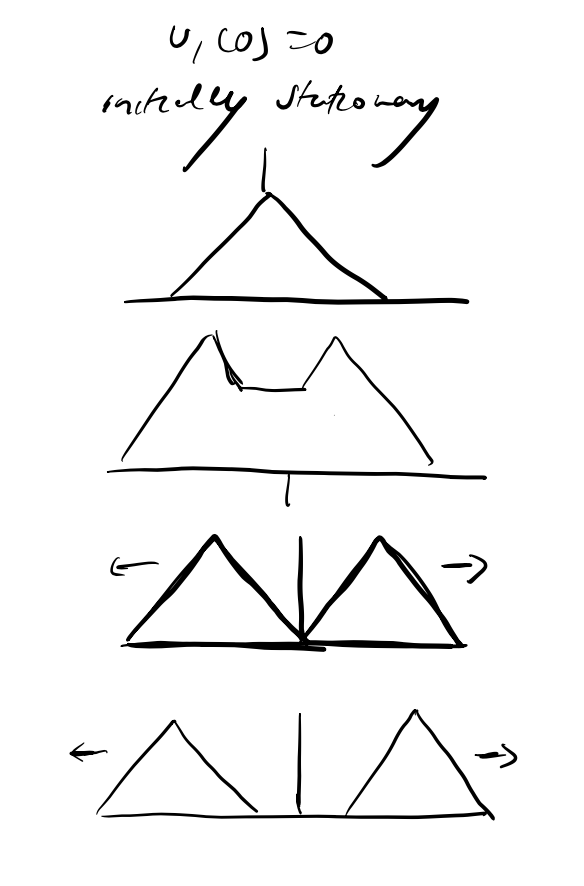
\includegraphics[width=0.45\textwidth]{waveevolution1.png} % jpg/png/pdf/eps
\end{figure}
For no initial condition but an initial velocity that is uniform in both directions we get
\begin{figure}[H]
	\centering
	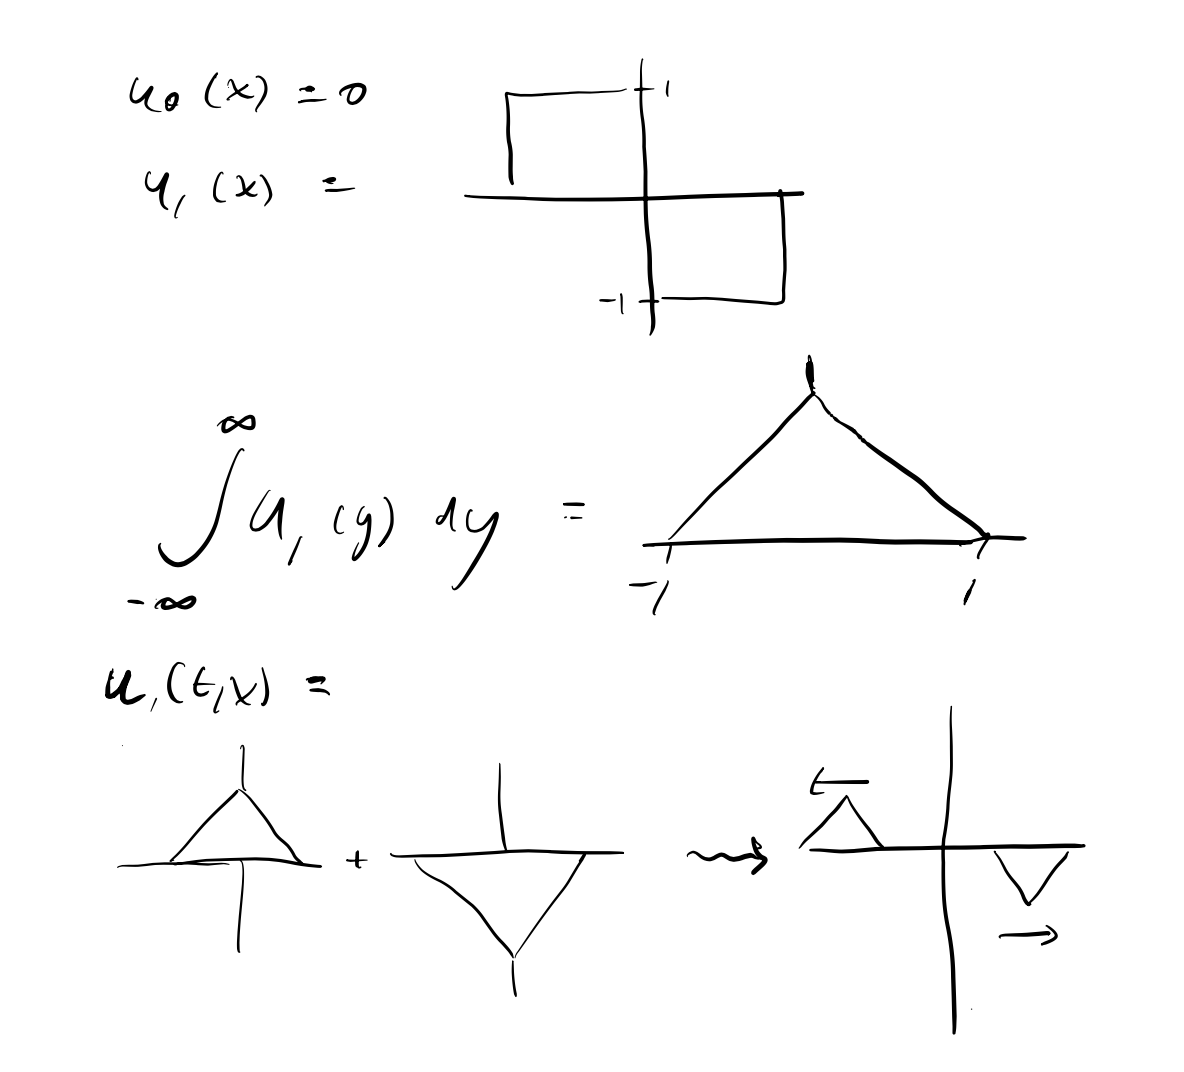
\includegraphics[width=0.65\textwidth]{waveevolution2.png} % jpg/png/pdf/eps
\end{figure}
 Now we will include a nontrivial $f(t,x)$
\begin{itemize}
\item $u_{tt}-u_{xx} = f(t,x)$
\item $u(0,x) = u_{0}(x)$
\item$u_{t}(0,x) = u_{1}(x)$
\end{itemize}
Because the operator as linear we can treat it as 3 different problems and take the sum of solutions to get the complete solution. First solution is
\begin{itemize}
	\item $u^{(1)}_{tt}-u^{(1)}_{xx} = f(t,x)$
	\item $u^{(1)}_{0}(x) = 0$
	\item$ u^{(1)}_{1}(x) = 0$
\end{itemize}
Second solution is
\begin{itemize}
	\item $u^{(2)}_{tt}-u^{(2)}_{xx} = 0$
	\item $u^{(2)}_{0}(x) = u_{0}(x)$
	\item$ u^{(2)}_{1}(x) = 0$
\end{itemize}
Third solution is
\begin{itemize}
	\item $u^{(3)}_{tt}-u^{(3)}_{xx} = 0$
	\item $u^{(3)}_{0}(x) = 0$
	\item$ u^{(3)}_{1}(x) = u_{1}(x)$
\end{itemize}
So
$$
u(t,x) = u^{(1)}(t,x) + u^{(2)}(t,x) + u^{(3)}(t,x)
$$
We already have the solution to the (2) and (3). Using the coordinates from earlier we have
$$
u_{\eta\xi} = -\frac{1}{4}f(\frac{\xi - \eta}{2},\frac{\xi + \eta}{2}) \Rightarrow u_{\xi} = C(\xi) - \int_{\eta_{0}(\xi)}^{\eta}\frac{1}{4}f(\frac{\xi - \eta^{\prime}}{2},\frac{\xi + \eta^{\prime}}{2})d\eta^{\prime}\Rightarrow
$$
$$
u(\eta,\xi) = C(\xi)+C(\eta) - \frac{1}{4}\int_{\xi_{0}}^{\xi}d\xi\int_{\eta_{0}}^{\eta}\frac{1}{4}f(\frac{\xi^{\prime} - \eta^{\prime}}{2},\frac{\xi^{\prime} + \eta^{\prime}}{2})d\eta^{\prime}
$$
\begin{center}
\textcolor{red}{Derive domain of integration, why are the constants 0}
\end{center}
Now we have
$$
u(\eta,\xi)=   \frac{1}{4}\int_{-\infty}^{\xi}d\xi\int_{\eta}^{\infty}\frac{1}{4}f(\frac{\xi^{\prime} - \eta^{\prime}}{2},\frac{\xi^{\prime} + \eta^{\prime}}{2})d\eta^{\prime}
$$
but we would like our solution in terms of original coordinates like the other two solutions.
\begin{center} \textcolor{red}{domain of integration again and change of variables}
\end{center}
$$
u^{(3)}(t,x) = \frac{1}{2}\int_{0}^{t}dt^{\prime}\int_{x-(t-t^{\prime})}^{x+(t-t^{\prime})}f(t^{\prime},x^{\prime})dx^{\prime}
$$
This expression does not carry over to higher dimensions, but gives us our general solution to the wave equation in (1+1) dimensions. 
\newline

Now we will study non-trivial boundary conditions. What is $u(t,x)$ when $x\in [0,\infty)$ with the same initial conditions $u_1$ and $u_2$. We have a couple of choices on what to do at the bondary. The first is the Dirichlett boundary condition where we fix the function at $x=0$ to a particular value. We could also allow the end to move. This is analgous to a the string tied to a ring around a pole at $x=0$. To do this we set $u_{x}(t,0) = 0$ so it cannot move in the x-direction, but still has the freedom to go up and down. We could even mix the boundary conditions for a more complicated problem, but these conditions occur infrequently in physical problems.
\newline

We can now apply a boundary condition to the general solution $u(x,t) = F(x+t)+G(x-t)$. 
$$
u(0,t) = 0 \Rightarrow F(t)+G(-t) = 0 \Rightarrow G(-t) = -F(t)
$$
This functional dependence suggest we use the method of reflections, similar to the method of images in electrostatics. We solve on the whole line with odd extensions of the initial data so that the boundary condition is built in. We originally had
\begin{itemize}
\item $u(0,x) =  u_{0}(x),\quad x\geq 0 $
\item $u_{t}(0,x) = u_{1}(x),\quad x\geq 0$
\end{itemize}
So we extend in the following way $u_{0}(-x) = -u_{0}(x)$ and $u_{1}(-x) = -u_{1}(x)$ when we let $x\in\mathbb{R}$. This is the same antisymmetry we have for the general solution on our restricted domain. So we can just use the solution on the whole domain with the new boundary conditions and then restrict that solution to $[0,\infty)$ to give us the solution we were originally looking for. Notice that $ u(t,-x)= -u(t,x)$ also satisfies our Dirichlett boundary condition.
	\lecture{4}{Wave Equation General Solution on a Manifold and more Boundary Conditions }
We take a detour from the main part of the course and study the $(1+1)$ wave equation with a general metric.
$$\sum_{i,j = 1}^{2}\frac{\partial}{\partial x^{i}}(a^{ij}(x^1,x^2)\frac{\partial u}{\partial x^{j}})=0, \quad \det{a^{ij}}<0$$
The metric is defined on a pseudoriemannian manifold $M$
$$
\sum_{i,j}g_{ij}(x^{1},x^{2})dx^{i}\otimes dx^{j}\in T^{*}M\otimes T^{*}M
$$
where $T^{*}M$ is the cotangent bundle of the manifold. These covectors are dual to the basis in our cotangent bundle
$$
dx^{i}(\frac{\partial}{\partial x^{j}}) = \delta^{i}_{\ j}
$$
and we have the inverse metric
$$
(g_{ij})^{-1} g^{ij} = \sum_{i,j}g^{ij}\frac{\partial}{\partial x^{i}}\otimes\frac{\partial}{\partial x^{j}} \in TM \otimes TM
$$
where $TM$ is the tangent bundle. It is easy to show that this is in fact the inverse of $g_{ij}$. We can use this to construct the general laplacian on a manifold (Laplace-Beltrami Operator)
\begin{align}
	\Delta_{g} u 
	= \frac{1}{\sqrt{|\det g|}}
	\sum_{i,j}
	\frac{\partial}{\partial x^{i}}
	\!\left(
	\sqrt{|\det g|}\, g^{ij}
	\frac{\partial u}{\partial x^{j}}
	\right).
\end{align}
It follows that in our wave equation
$$
a^{ij} = \sqrt{|\det{g}|}g^{ij}
$$
To simplify the form of this equation we would like to find a change of coordinates that such that $g_{ij}dx^{i}dx^{j}\to 2f(\xi,\eta)d\xi d\eta$ like the simpification we did at the beginning of lecture 3 in Euclidean space. This allowed us to find the general solution in terms of specified initial conditions. If this is the case the metric will have the form
$$
g_{ij} = 
\begin{pmatrix}
	0 & f\\
	f & 0
\end{pmatrix}, \quad \sqrt{|\det{g}|} = f \Rightarrow a^{ij} = \begin{pmatrix}
0 & 1\\
1& 0
\end{pmatrix}
$$
So our wave equation on a manifold simplifies to 
$$ \frac{1}{f}\partial_{\xi}\partial_{\eta} u = 0$$
Let us try to understand why this works. First consider the metric acting on a vector and try to solve for the vectors that are annhilated by it.
$$
\sum_{i,j}g_{ij}dx^{i}dx^{j}(\sum_{k}v^{k}\frac{\partial}{\partial x^{k}}) = \sum_{i,j}g_{ij}v^{i}v^{j} = 0 \Leftrightarrow (v^{1})^{2}-(v^{2})^{2} = 0
$$
Integrating these vectors along a path describes light-like geodesics like General Relativity. \begin{figure}[H]
	\centering
	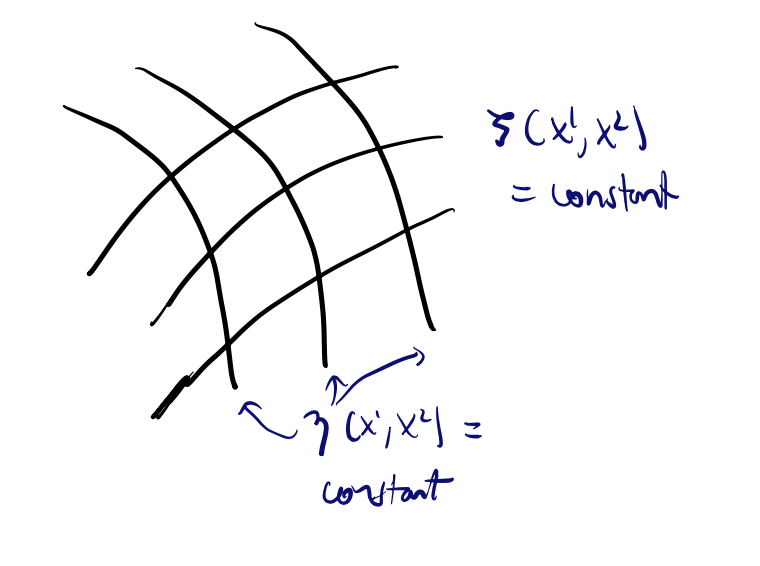
\includegraphics[width=0.65\textwidth]{desiredcoordinates.png} % jpg/png/pdf/eps
\end{figure}
$\xi$ and $\eta$ are our preferred coordinates that simplify the metric. The metric is 0 along the curves. Let us consider an example metric where we find the desired change of coordinates. There is an example in the video from minutes 31-58. But its a bit above the scope of this class, so we leave it out.
Now we return to the boundary conditions we were studying at the end of lecture 3. 
\begin{figure}[H]
	\centering
	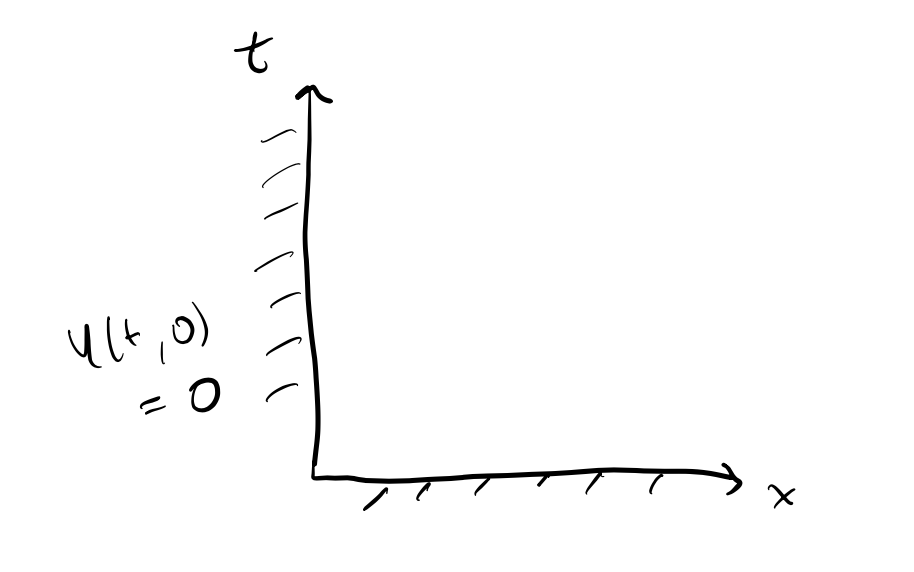
\includegraphics[width=0.4\textwidth]{dirichlett.png} % jpg/png/pdf/eps
\end{figure}
and set $u(t,0)=0$, the Dirichlett boundary condition. To find the solution to this restricted domain, we extend the solution to all of $\mathbb{R}$ by
$$
u(t,x) = -u(t,-x)
$$
We now have a mirror image on the opposite side of our boundary at $x=0$.
\begin{figure}[H]
	\centering
	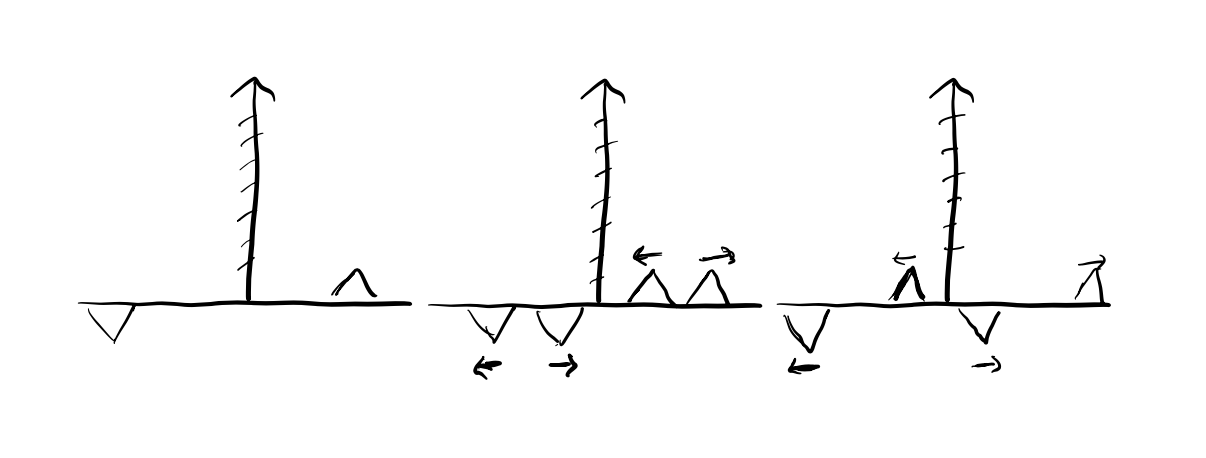
\includegraphics[width=0.6\textwidth]{reflection.png} % jpg/png/pdf/eps
\end{figure}
We now consider the Von Neumann boundary condition. Similar to the image above, we set $u_{x}(t,0) = 0$ and extend with 
$$
u(t,-x) = u(t,x)
$$
Taking the derivatives of both side of this extension equation we can see that the extension agrees at the boundary with our solution on the restricted domain. Now we have solutions like
\begin{figure}[H]
	\centering
	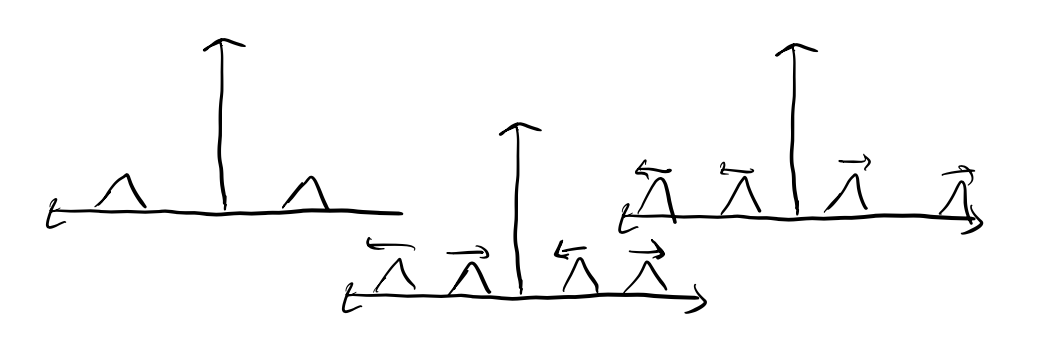
\includegraphics[width=0.6\textwidth]{vn.png} % jpg/png/pdf/eps
\end{figure}
Another interesting case are periodic and antiperiodic boundary conditions. These are described on a periodic system by $u(t,x+L)= \pm u(t,x)$. 
\begin{figure}[H]
	\centering
	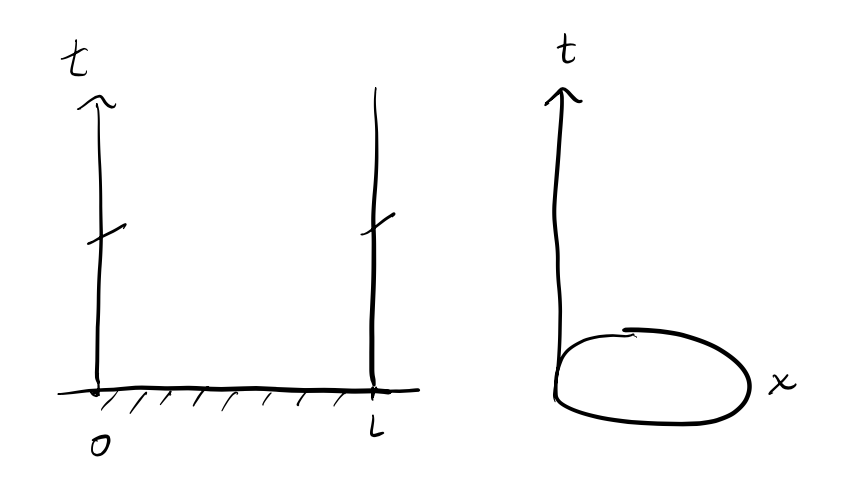
\includegraphics[width=0.6\textwidth]{pbc.png} % jpg/png/pdf/eps
\end{figure}

We start with antiperiodic solutions because we can use them to build periodic solutions by doubling the interval. Recall $u(x,t) = F(x+t)+G(x-t)$. with initial conditions $F(x)+G(x) = u_{0}(x)$ and $F^{\prime}(x)-G^{\prime}(x)= u_{1}(x)$. These conditions are on $x\in[0,L]$ but we can extend them with our periodic conditions $u_{0}(x+L) = u_{0}(x)$ and $u_{1}(x+L) = u_{1}(x)$. When we perform the integral of $u_{1}(x)$ it will break periodicity because it will receive some extra shift. We can fix this by defining
$$
\tilde{u}(x,t) = u(x,t)+ct
$$
We have the same initial conditions for this problem except $\tilde{u}_{1}(x) = u_{1}(x)+c$. Now we can solve
$$
\int_{x}^{x+L}\tilde{u}_{1}(x)dx = \int_{x}^{x+L}u_{1}(x)dx + cL = 0
$$
\begin{figure}[H]
	\centering
	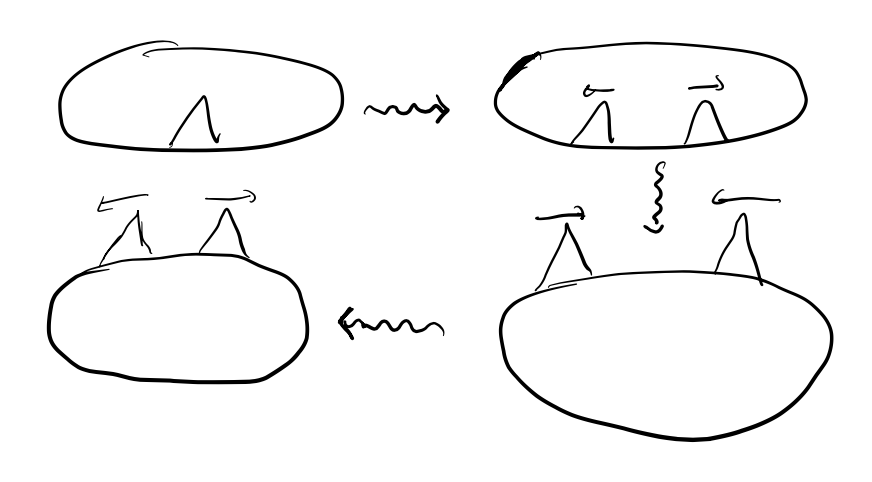
\includegraphics[width=0.6\textwidth]{onaring.png} % jpg/png/pdf/eps
\end{figure}
This case is interesting because we can use it to combine two boundary conditions. We use these the conditions
\begin{enumerate}
\item $u(t,x)=u(t,x+L)$
\item $u(t,-x) = -u(t,x)$
\end{enumerate}
This is equivalent to Dirichlett boundary conditions on the interval $[0,L/2]$
\begin{figure}[H]
	\centering
	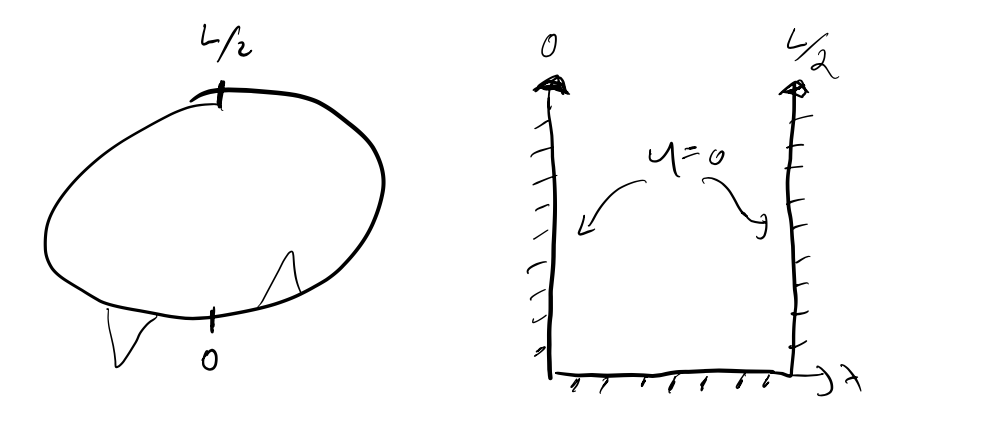
\includegraphics[width=0.6\textwidth]{equaldirichlett.png} % jpg/png/pdf/eps
\end{figure}
\problems{
\begin{exercise}
	Check that the general solution of the equation
	\[
	\partial_x\!\left( \frac{xy}{x^2 + y^2} \, \partial_x u \right)
	+ \frac{1}{2}\partial_x\!\left( \frac{x^2 - y^2}{x^2 + y^2} \, \partial_y u \right)
	+ \frac{1}{2}\partial_y\!\left( \frac{x^2 - y^2}{x^2 + y^2} \, \partial_x u \right)
	- \partial_y\!\left( \frac{xy}{x^2 + y^2} \, \partial_y u \right) = 0
	\]
	is given by
	\[
	u(x, y) = F(x^2 - y^2) + G(xy).
	\]
\end{exercise}

\begin{exercise}
	Solve the wave equation:
	\[
	u_{tt} - u_{xx} = f(t, x), \quad u(0, x) = u_t(0, x) = 0,
	\]
	where
	\[
	f(t, x) = (\theta_H(t - 1) - \theta_H(t - 3)) \, (\theta_H(x + 1) - \theta_H(x - 1)).
	\]
\end{exercise}

\begin{exercise}
	Solve the wave equation in $\mathbb{R}^{1+1}$:
	\[
	u_{tt} - u_{xx} = \theta_H(x + 3) - 2\theta_H(x + 2) + 2\theta_H(x - 2) - \theta_H(x - 3),
	\quad u(0, x) = u_t(0, x) = 0.
	\]
	You may first consider the case $t > 4$, and then obtain the solution for arbitrary $t$.
\end{exercise}
\begin{exercise}
	Solve the wave equation $u_{tt} - u_{xx} = 0$ on $\mathbb{R}$ with the following initial conditions:
	\[
	u_t(0, x) = |1 - x^2|\theta_H(1 - x^2), \qquad u(0, x) = 0,
	\]
	where $\theta_H(x) = 0$ for $x \le 0$ and $\theta_H(x) = 1$ for $x > 0$.  
	Plot this solution for some values of $t$.
\end{exercise}

\begin{exercise}
	Solve the equation
	\[
	u_{tt} - 2u_{xx} - u_{tx} = 0, \quad u_t(0, x) = 0, \quad u(0, x) = (1 - x^2)\theta_H(1 - x^2).
	\]
\end{exercise}


}
\lecture{5}{End of wave equation boundary problems (time dependent) and General Strategies for PDEs (Greens Function)}
To finish off boundary conditions for the wave equation, let us consider time dependent boundary conditions for
$$
u_{tt}-u_{xx}=0
$$
We have the same initial conditions supplied but now a constraint at the boundary
\begin{figure}[H]
	\centering
	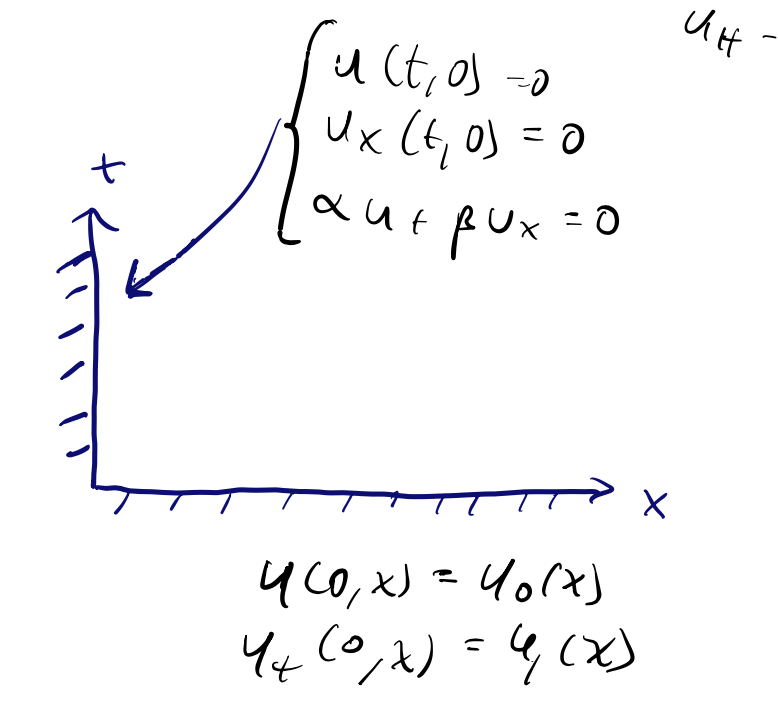
\includegraphics[width=0.65\textwidth]{time1.png} % jpg/png/pdf/eps
\end{figure}
We could even consider two boundaries
\begin{figure}[H]
	\centering
	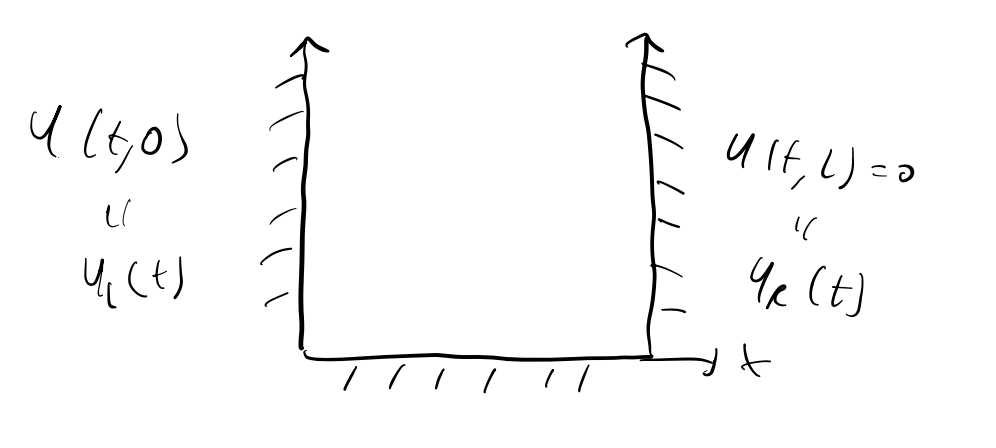
\includegraphics[width=0.65\textwidth]{time2.png} % jpg/png/pdf/eps
\end{figure}
The strategy is to try and reduce it to a problem we know how to solve. We can transfer the boundary conditions to the right hand side by defining
$$
\tilde{u}(t,x) = u(t,x)-\frac{x}{L}u_{R}(t)-(1-\frac{x}{L})u_{L}(t)
$$
One can easily check that 
$$
\tilde{u}(t,0)-\tilde{u}(t,L)=0
$$
Now our wave equation with the new function becomes
$$
\tilde{u}_{tt}-\tilde{u}_{xx} = (u_{tt}-u_{xx})-\frac{x}{L}u^{\prime\prime}_{R}(t)-(1-\frac{x}{L})u^{\prime\prime}_{L}(t) = -\frac{x}{L}u^{\prime\prime}_{R}(t)-(1-\frac{x}{L})u^{\prime\prime}_{L}(t)
$$
\textcolor{red}{I don't understand this strategy} The second strategy is to use our known solution on the real line and match it to the boundary condition, so when we restrict the domain it give us the solution we desire.
\begin{figure}[H]
	\centering
	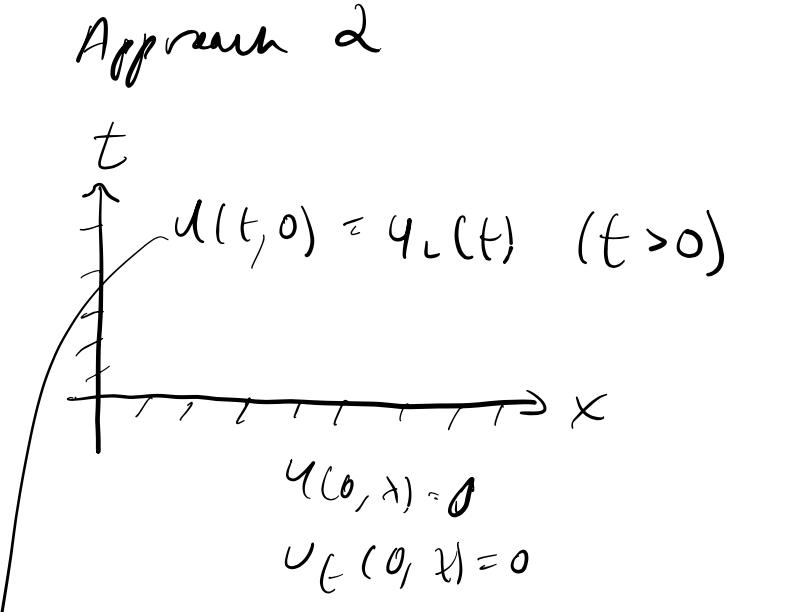
\includegraphics[width=0.65\textwidth]{Approach2.png} % jpg/png/pdf/eps
\end{figure}
Recall the general solution on the real line had the form
$$
u(t,x) =  F(t-x)+G(t+x)
$$
We can now define this for $u_{L}(t)=0$ for $t<0$. The wave will enter from the left and always match our boundary condition. We notice that taking spatial derivatives of our general form flips the sign. 
\textcolor{red}{fill in the rest of this derivation from video}
$$
u(t,x) = u_{L}(t-x)
$$
\begin{itemize}
\item solution to our wave equation
\item $u(t,0) = u_{L}(t)$
\item $u(t=0,x) = u(0,x) = u_{L}(-x), x>0$
\item$u_{t}(0,x) = u_{L}^{\prime}(-x)$
\end{itemize}
\begin{figure}[H]
	\centering
	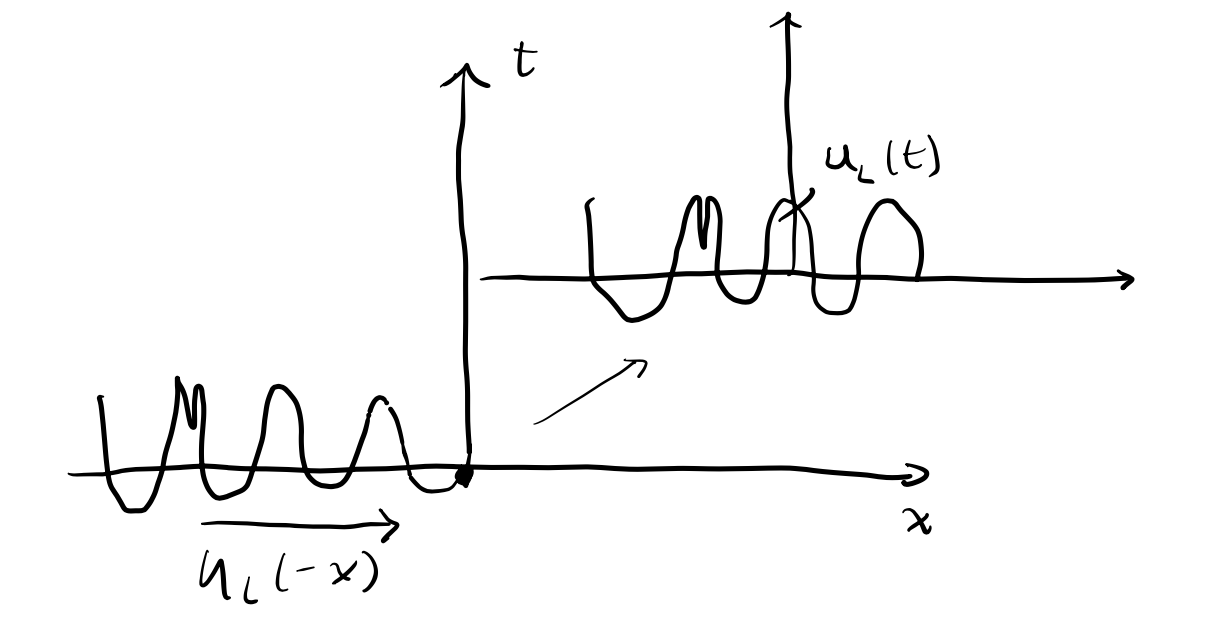
\includegraphics[width=0.65\textwidth]{fromLeft.png} % jpg/png/pdf/eps
\end{figure}
This ends our discussion on the $(1+1)$ wave equation. Now we transition to general strategies for solving PDEs.
The three main stratgeies are
\begin{enumerate}
\item Just solve it like we have done with the wave equation by integrating
\item Find a Green's function to undo the operator
\item Fourier Transform to get a more easily solvable form
\end{enumerate}
In $(1+1)$ dimensions for a driven wave on $\mathbb{R}$ we had 
$$
u(t,x) = \frac{1}{2}\int_{0}^{t}dt^{\prime}\int_{x-|t-t^{\prime}|}^{x+|t-t^{\prime}|}dx^{\prime}f(t^{\prime},x^{\prime})
$$
We expect this to generalize to $1+d$ with
$$
u(t,\vec{x})= \frac{1}{2}\int_{\mathbb{R}^{d+1}}dt^{\prime}d\vec{x}^{\prime}G(t,\vec{x};t^{\prime},\vec{x}^{\prime}) f(t^{\prime},\vec{x}^{\prime})
$$
We can read off the explicit form of the green's function from the integral solution. Recall the the Heaviside function $\theta_{H}(x)$ is defined as
\[
\theta_H(x) =
\begin{cases}
	0, & x < 0, \\
	\frac{1}{2}, & x = 0, \\
	1, & x > 0.
\end{cases}
\]
For $d+1$ we have
$$
G(t,x;t^{\prime},x^{\prime}) = \frac{1}{2}\theta_{H}(t-t^{\prime})\theta_{H}(t^{\prime})[\theta_{H}(x-x^{\prime}+|t-t^{\prime}|)-\theta_{H}(x-x^{\prime}-|t-t^{\prime}|)]
$$
\textcolor{red}{Exercise: check that this is describing the function over the domain of integration} This shows us that our Green's functio approach matches our integration approach. To understand the Green's function better let us study the discretization of 
$$
u_{tt}-\Delta u +\alpha u = f
$$
on a periodic boundary.
\begin{figure}[H]
	\centering
	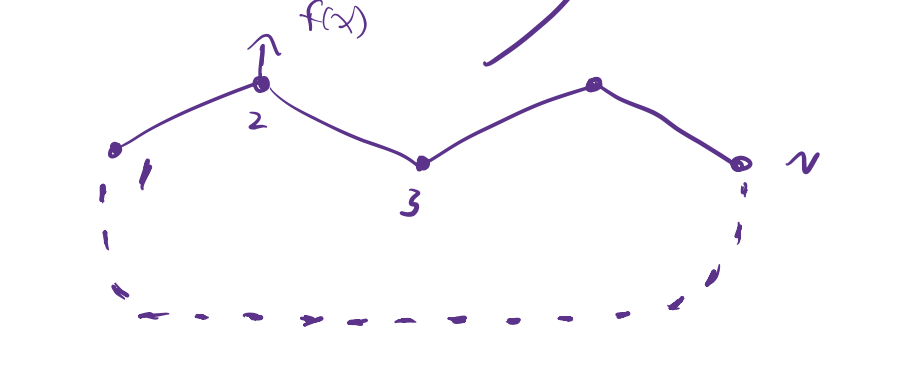
\includegraphics[width=0.65\textwidth]{periodicchain.png} % jpg/png/pdf/eps
\end{figure}
We identify $f(N+1)\sim f(1)$. The discrete version of this equation is
$$
-u(t,x+1)+ 2u(t,x)-u(t,x-1)+\alpha u(t,x) = f(x)
$$
Neglecting time dependence will simplify the problem. So we are solving for a stationary state.
For $x\in\{1,...,N\}$ we have
$$
-u(x+1) + 2u(x)-u(x-1)+\alpha u(x) = f(x)
$$
If we have $\vec{u}=[u(1),...,u(N)]^{T}$ and $\vec{f} = [f(1),...,f(N)]^{T}$ then the corresponding matrix is
\[
A =
\begin{pmatrix}
	2+\alpha & -1        & 0         & \cdots  & 0         & -1 \\
	-1        & 2+\alpha & -1        & \cdots  & 0         & 0  \\
	0         & -1        & 2+\alpha & \ddots  & \vdots    & \vdots \\
	\vdots    & \ddots   & \ddots    & \ddots  & -1        & 0 \\
	0         & 0         & \cdots   & -1      & 2+\alpha  & -1 \\
	-1        & 0         & \cdots   & 0       & -1        & 2+\alpha
\end{pmatrix}
\]
for the equation $T\vec{u} = \vec{f}$. So $T\sim \tilde{\alpha}-\tilde{\Delta}$. The solution for $\vec{u}$ is found by inverting this matrix. This is the greens function for a finite dimensional system.
$$
\vec{u} = (\alpha-\Delta)^{-1}\vec{f}=G\vec{f}
$$
We can express $G$ as a matrix
\[
G =
\begin{pmatrix}
	G(1,1) & G(1,2) & G(1,3) & \cdots & G(1,N) \\
	G(2,1) & G(2,2) & G(2,3) & \cdots & G(2,N) \\
	G(3,1) & G(3,2) & G(3,3) & \cdots & G(3,N) \\
	\vdots & \vdots & \vdots & \ddots & \vdots \\
	G(N,1) & G(N,2) & G(N,3) & \cdots & G(N,N)
\end{pmatrix}
\]
This gives us
$$
u(x)=\sum_{x^{\prime}}^{N}G(x,x^{\prime})f(x^{\prime})$$
we compare this with the earlier solution
$$
\vec{u}(t,\vec{x})= \frac{1}{2}\int_{\mathbb{R}^{d+1}}dt^{\prime}d\vec{x}^{\prime}G(t,\vec{x};t^{\prime},\vec{x}^{\prime}) f(t^{\prime},\vec{x}^{\prime})
$$ 
and note the similarities
\begin{enumerate}
\item $x^{\prime}\leftrightarrow(t^{\prime},\vec{x}^{\prime})$	
\item $\sum_{x^{\prime}}\leftrightarrow \int dt^{\prime}d\vec{x}^{\prime}$
\item $G(x,x^{\prime})\leftrightarrow G(t,x;t^{\prime},x^{\prime})$
\end{enumerate}
The equation satisfied by the greens function is 
$$
(\alpha-\Delta)\cdot G = \mathbb{I} \Leftrightarrow [(\alpha-\Delta)\cdot G](x,x^{\prime}) = \delta_{x,x^{\prime}}
$$
For a particular $x_{0}$ we have
$$
-G(x_{0}+1,x^{\prime})+(\alpha+2)G(x_{0},x^{\prime})-G(x_{0}-1,x^{\prime})= \delta_{x_{0},x^{\prime}}
$$
We see this is exactly the same equation as earlier but $f(x)$ has been replaced by a delta function. This is drastically simpler. Now we have $f(x_{0}) = [0,...,1,....,0]^{T}$ with 1 at the $x_{0}^{\text{th}}$ position
We can expand out $f(x)$ by
$$
f(x) = \sum_{x^{\prime}}^{N}\delta_{x,x^{\prime}}f(x^{\prime})
$$
Using linearity we have

\begin{align*}
	(\alpha I - \Delta_x)\,u(x)
	&= (\alpha I - \Delta_x)\sum_{x'=1}^N G(x,x')\,f(x') \\
	&= \sum_{x'=1}^N \bigl[(\alpha I - \Delta_x)G(x,x')\bigr]\,f(x') \\
	&= \sum_{x'=1}^N \delta_{x,x'}\,f(x') \\
	&= f(x).
\end{align*}
We see that the Green's function is the inverse of the operator satisfies a much simpler equation 
$$
(\alpha - \Delta_{x})G(x,x^{\prime})=\delta_{x,x^{\prime}}
$$
or 
$$
(\partial_{t}^{2}-\Delta)G(t,\vec{x};t^{\prime},x^{\prime}) = \delta(t-t^{\prime})\delta^{(d)}(\vec{x}-\vec{x}^{\prime})
$$
The Greens function has the same form in the discrete case and the continuous case.
There are two ways to get the greens functions. We can just solve the equation. But another approach is to use the Fourier transform.
\begin{figure}[H]
	\centering
	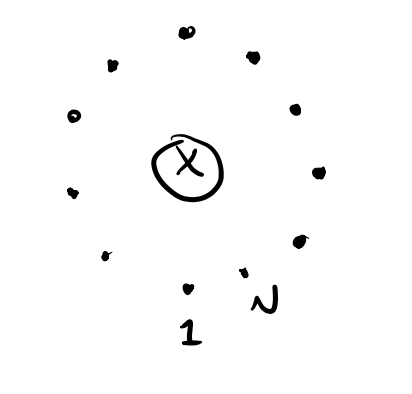
\includegraphics[width=0.3\textwidth]{FT1.png} % jpg/png/pdf/eps
\end{figure}
Notice that our system has rotational symmetry. $f(x)\mapsto f(x+1)$ or in matrix notation $f(x)\mapsto Tf(x)$ where $T$ is the shift operator
\[
T=
\begin{pmatrix}
	0 & 1 & 0 & \cdots & 0 \\
	0 & 0 & 1 & \cdots & 0 \\
	\vdots & \ddots & \ddots & \ddots & \vdots \\
	0 & \cdots & 0 & 0 & 1 \\
	1 & 0 & \cdots & 0 & 0
\end{pmatrix}
\]
and the obvious inverse
 \[
T^{-1} =
\begin{pmatrix}
	0 & 0 & \cdots & 0 & 1 \\
	1 & 0 & \cdots & 0 & 0 \\
	0 & 1 & \ddots & \vdots & \vdots \\
	\vdots & \ddots & \ddots & 0 & 0 \\
	0 & \cdots & 0 & 1 & 0
\end{pmatrix}
\]
We can use these matrices and the identity to write the earlier operator.
$$
\alpha - \Delta = (2+\alpha)\mathbb{I}-(T+T^{-1}
)$$
We need to compute the inverse matrix which is always easier in the diaganol eigenfunction basis. Let us diaganolize $T$. We need to solve the eigenvalue equation
$$
T\varphi_{k}(x)=\lambda_{k}\varphi_{k}(x)\Leftrightarrow \varphi_{k}(x+1) = \lambda_{k}\varphi(x)
$$
Because the lattice is periodic we have $T^{N} = \mathbb{I}$. So we conclude 
$$
\lambda_{k}^{N} = 1
$$
This is simply the equation for roots of unity. We deduce that the eigenfunctions are
$$
\varphi_{k}(x)  =\frac{1}{\sqrt{N}} e^{\frac{2\pi i kx}{N}}
$$
In this way we have found the beautiful result that connects the fourier basis of the discrete fourier transform to eigenvalues of the shift operator. This transform arose from other symmetries of our system. If we had a different kind of symmetry it is possible to diaganolize via a different type of transform.
\problems{
	\begin{exercise}
		Solve the wave equation on a half-line $x > 0$:
		\[
		u_{tt} - u_{xx} = 0, \quad u(0, x) = 0, \quad u_t(0, x) = \theta_H(x - 3) - \theta_H(x - 2), \quad u(t, 0) = 0.
		\]
		For simplicity, consider only the large time case.
	\end{exercise}
	\begin{exercise}
		Solve the wave equation $u_{tt} - u_{xx} = 0$ on $\mathbb{R}_{>0}$ with the following initial and boundary conditions:
		\[
		u_t(0, x) = 0, \quad u(0, x) = \sin^2(2\pi x)\theta_H(1 - |x - 2|), \quad
		u(t, 0) = \tfrac{1}{2}\sin^2(2\pi t)\theta_H(1 - |t - 2|).
		\]
		Plot this solution for some values of $t$.
	\end{exercise}
	\begin{exercise}
		Solve the wave equation on a half-line $x > 0$:
		\[
		u_{tt} - u_{xx} = \theta_H(1 - x), \quad u(0, x) = 0, \quad u_t(0, x) = 0, \quad u(t, 0) = 0,
		\]
		where $\theta_H$ is the Heaviside theta function:
		\[
		\theta_H(x) =
		\begin{cases}
			0, & x < 0, \\
			1, & x > 0, \\
			\frac{1}{2}, & x = 0.
		\end{cases}
		\]
		For simplicity, consider its solution only for $t > 4$.
	\end{exercise}
\begin{exercise}
	Find the Green function of the discrete Laplace operator on a finite lattice with periodic boundary conditions $(\mathbb{Z}/N\mathbb{Z})$, $\Delta = T + T^{-1} - 2$.  
	Solve this problem directly, then check that the obtained result is consistent with the Fourier transform.
\end{exercise}
\begin{exercise}
	Solve the following initial and boundary value problems on the rectangle $x \in [0, L]$, $t \in [0, T]$, with zero boundary conditions $u(t, 0) = u(t, L) = 0$:
	\[
	\begin{cases}
		u_{tt}(t, x) - u_{xx}(t, x) = 0, & u(0, x) = \sin^3 \frac{\pi x}{L}, \; u_t(0, x) = \sin \frac{2\pi x}{L}, \\
		u_{tt}(t, x) + u_{xx}(t, x) = 0, & u(0, x) = \sin \frac{\pi x}{L}, \; u(T, x) = \sin^3 \frac{\pi x}{L}.
	\end{cases}
	\]
\end{exercise}
}
\lecture{6}{General Strategies Continued (Fourier Transform)}
Now we continue our studyt of the fourier transform. For $(\alpha-\Delta)u$, the greens function is
$$
G(x,x^{\prime}) = (\alpha-\Delta)^{-1}(x,x^{\prime})
$$
Previously we found the diaganol basis
$$
\varphi_{k}(x)  =\frac{1}{\sqrt{N}} e^{\frac{2\pi i kx}{N}}
$$
Using this and the previous result $(\alpha-\Delta) = (2+\alpha)-(T+T^{-1})$ we get
$$
(\alpha - \Delta)\varphi_{k} = \Big[2+\alpha + -e^{\frac{2\pi i k }{N}}-e^{-\frac{2\pi i k }{N}}\Big]\varphi_{k}
$$
We can expand 
$$
f(x)=\frac{1}{\sqrt{N}}\sum_{k=1}^{N}e^{\frac{2\pi i kx}{N}}\tilde{f}(k)
$$
The transform goes maps between two periodic lattices $\mathbb{Z}/N\mathbb{Z}\leftrightarrow \mathbb{Z}/N\mathbb{Z}$
\begin{figure}[H]
	\centering
	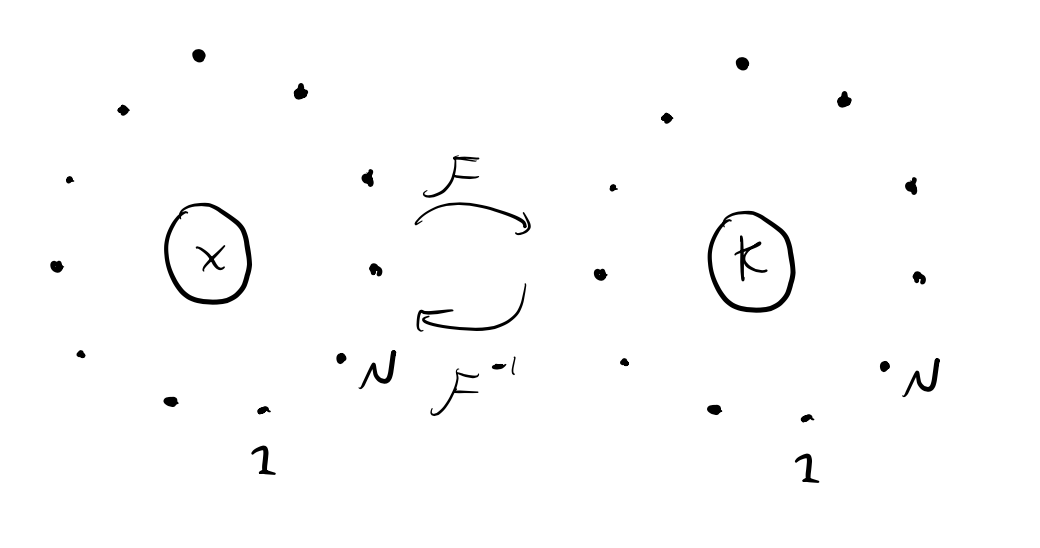
\includegraphics[width=0.5\textwidth]{FT2.png} % jpg/png/pdf/eps
\end{figure}
We will later study transforms between $\mathbb{Z}\leftrightarrow S^{1}$ and $\mathbb{R}\leftrightarrow\mathbb{R}$. We can derive the inverse transform from the orthogonality condition
$$
\tilde{f}(k)=\frac{1}{\sqrt{N}}\sum_{x=1}^{N}f(x)e^{-\frac{2 \pi i k x}{N}}
$$
It is easy to compute the sum when $k=k^{\prime}$.
For \(k \neq k'\), let \(m = k' - k \neq 0\). Then
\[
\sum_{x=1}^{N} e^{2\pi i (k'-k)x / N}
= \sum_{x=1}^{N} \left(e^{2\pi i m / N}\right)^x
= \frac{1 - \left(e^{2\pi i m / N}\right)^{N}}{1 - e^{2\pi i m / N}}.
\]
where we have calculated the geometric series. Since \(e^{2\pi i m} = 1\), the numerator vanishes:
\[
1 - \left(e^{2\pi i m / N}\right)^{N} = 1 - e^{2\pi i m} = 0.
\]
Hence the sum equals zero:
we conclude that the basis functions $\{\varphi_{k}\}$ form an orthogonal set. We can understand these results through matrix representations.
$$
\Omega(x,y)  =
\frac{1}{\sqrt{N}}
\begin{pmatrix}
	e^{\frac{2\pi i (1)(1)}{N}} & e^{\frac{2\pi i (1)(2)}{N}} & \cdots & e^{\frac{2\pi i (1)(N-1)}{N}} & 1 \\[4pt]
	e^{\frac{2\pi i (2)(1)}{N}} & e^{\frac{2\pi i (2)(2)}{N}} & \cdots & e^{\frac{2\pi i (2)(N-1)}{N}} & 1 \\[4pt]
	\vdots & \vdots & \ddots & \vdots & \vdots \\[4pt]
	e^{\frac{2\pi i (N-1)(1)}{N}} & e^{\frac{2\pi i (N-1)(2)}{N}} & \cdots & e^{\frac{2\pi i (N-1)(N-1)}{N}} & 1 \\[4pt]
	1 & 1 & \cdots & 1 & 1
\end{pmatrix}
$$
It is easy to check that $\Omega(x,y)^{\dagger}\Omega(x,y) = \mathbb{I}$. We see that it is a unitary transformation which is cruical in physics. But this unitarity depends on the geometry of the underlying space.  We derive a few more properties of the discrete fourier transform
\begin{itemize}
\item reality: $f(x)^{*} = f(x)$
\item $\tilde{f}(N-k)^{*} = \tilde{f}(k) \Rightarrow \tilde{f}(N)^{*} = \tilde{f}(N)$
\item $(f,g) = (\tilde{f},\tilde{g})$
\end{itemize}
The second point shows us that all the point on the periodic lattice are reflected under the complex conjugation process. The third point is that the scalar produce is presereved because of the unitarity mentioned earlier. Now we can return to finding the greens function with our results.
$$
\Big(\frac{1}{\alpha-\Delta}f\Big)(x) = \frac{1}{\alpha-\Delta}\frac{1}{\sqrt{N}}\sum_{k=1}^{N}e^{\frac{2\pi i k x}{N}}\tilde{f}(k) =  \frac{1}{\sqrt{N}}\sum_{k=1}^{N}e^{\frac{2\pi i k x}{N}}\frac{1}{\lambda(k)}\tilde{f}(k) = 
$$
$$
\frac{1}{N}\sum_{k=1}^{N}\sum_{x^{\prime}}e^{\frac{2\pi i k x}{N}}\frac{1}{\lambda(k)}e^{-\frac{2\pi i k x^{\prime}}{N}}f(x^{\prime}) = \sum_{x^{\prime}=1}^{N}G(x,x^{\prime})f(x^{\prime})
$$
where $G(x,x^{\prime})= G(x-x^{\prime}) = \frac{1}{N}\sum_{k=1}^{N}\frac{1}{\lambda(k)}e^{\frac{2\pi ik(x-x^{\prime})}{N}}$. So we can use this technique to help us find our green's function in discrete position space with $\lambda(k)$ being the dispersion relation for the operator, $1/\lambda(k)$ being th propogator in momentum space. This diagnolize-solve-transform back works for linear operators all over mathematical physics.
\newline

Pavlo derives the convolution when we transform the product of two functions, which is interesting, but I omit the derivation. When we take the Fourier transform of a product of two discrete periodic functions we get
\[
(f * g)(x)
= \frac{1}{N} \sum_{x'=1}^{N} f(x')\, g(x - x')
\]
where subtraction $(x - x')$ is taken modulo $N$ to enforce periodicity. Its as if we expand each function in its own modes, then multiply all the other functions modes by all of these to get the new weights $f(x^{\prime})g(x-x^{\prime})$
All of these properties carry over to the two other fourier transforms we can study with their continuous analogs.
\begin{itemize}
	\item $\mathbb{R} \leftrightarrow \mathbb{R}$
	\[
	\tilde{f}(k) = \frac{1}{\sqrt{2\pi}} \int_{-\infty}^{\infty} f(x)\, e^{-i k x}\, dx,
	\qquad
	f(x) = \frac{1}{\sqrt{2\pi}} \int_{-\infty}^{\infty} \tilde{f}(k)\, e^{i k x}\, dk.
	\]
	
	\item $S^{1} \leftrightarrow \mathbb{Z}$
	\[
	\tilde{f}_{n} = \frac{1}{2\pi} \int_{0}^{2\pi} f(\theta)\, e^{-i n \theta}\, d\theta,
	\qquad
	f(\theta) = \sum_{n \in \mathbb{Z}} \tilde{f}_{n}\, e^{i n \theta}.
	\]
\end{itemize}
The lecture ends explaing that the dirac delta function is the continuum limit of the kronecker delta function.
\problems{
\begin{exercise}
	Study the Fourier transform on a segment $x = 1, \dots, N$:
	\begin{enumerate}
		\item Compute scalar products between the functions $\varphi_k(x) = \sin\frac{\pi kx}{N+1}$, $k = 1, \dots, N$:
		\[
		(\varphi_k, \varphi_{k'}) = \sum_{x=1}^{N} \varphi_k(x)\varphi_{k'}(x).
		\]
		\item Write the formulas for the direct and inverse Fourier transform.
	\end{enumerate}
\end{exercise}
\solution{
	\begin{enumerate}
		\item This is a fourier transform on a discrete line segment $[0,L]$ broken up into $N$ points. 
We have the scalar product
$$
(\varphi_{k},\varphi_{k^{\prime}}) = \frac{1}{2}\sum_{x=1}^{N}\cos{\big(\frac{\pi(k-k^{\prime})x}{N+1}\big)}- \frac{1}{2}\sum_{x=1}^{N}\cos{\big(\frac{\pi(k+k^{\prime})x}{N+1}\big)}
$$
Let us consider when $k=k^{\prime}$. The first is just $N/2$. What is the second sum? We rewrite it as a geometric series  to get
$$
-\frac{1}{2}\sum_{x=1}^{N}\Re{e^{i\frac{2\pi k}{N+1}x}} = -\frac{1}{2}\sum_{x=0}^{N}\Re{e^{i\frac{2\pi k}{N+1}x}}+\frac{1}{2} = -\frac{1}{2}\Re{\frac{1-e^{i2\pi k}}{1-e^{\frac{i2\pi k}{N+1}}}}+\frac{1}{2} = 0 +\frac{1}{2}
$$
So for all $k = k^{\prime}$ we have
$$
(\varphi_{k},\varphi_{k^{\prime}}) = \frac{N+1}{2}$$
Now let us do the series for $k\neq k^{\prime}$
$$
\frac{1}{2}\big[\sum_{x=0}^{N}\Re{e^{i\frac{\pi (k-k^{\prime})}{N+1}x}}- \sum_{x=0}^{N}\Re{e^{i\frac{\pi (k+k^{\prime})}{N+1}x}}\big] = \frac{1}{2}\Re{\bigg[\frac{1-e^{i\pi(k-k^{\prime})}}{1-e^{\frac{i\pi (k-k^{\prime})}{N+1}}}-\frac{1-e^{i\pi(k+k^{\prime})}}{1-e^{\frac{i\pi (k+k^{\prime})}{N+1}}}\bigg]} = 0
$$
If the powers are odd then we have $2-2 = 0$. If powers are even then we have $0-0 = 0$. In conclusion we have
$$
(\varphi_{k},\varphi_{k^{\prime}}) = \frac{N+1}{2}\delta_{k,k^{\prime}}
$$
\item Now we must find the fourier transform and its inverse because the functions are orthogonal on $\{1,...,N\}$ we should have
\begin{itemize}
\item $\tilde{f}(k) = \sqrt{\frac{2}{N+1}}\sum_{x=1}^{N}f(x)\sin{(\frac{\pi k x}{N+1})}$
\item $f(x) = \sqrt{\frac{2}{N+1}}\sum_{k=1}^{N}\tilde{f}(k)\sin{(\frac{\pi k x}{N+1})}$
\end{itemize}
\end{enumerate}
}

\begin{exercise}
	Compute the Fourier transforms of the following functions on the real line:
	\[
	f_3(x) = \frac{1}{\cosh x}, \qquad f_4(x) = (1 - 2x^2)e^{-x^2/2}.
	\]
\end{exercise}
\solution{
\begin{itemize}
\item $\tilde{f}_{3}(p) = \int_{-\infty}^{\infty}\frac{e^{ipx}}{\cosh{(x)}}dx$ We have $\cosh{(x)} = \frac{e^{x}+e^{-x}}{2} = 0 \Leftrightarrow x = i\pi\frac{k}{2}+in\pi, n\in\mathbb{Z}$.
We can find the integral by doing a contour intergal in the complex plane
$$
\oint \frac{e^{ipz}}{\cosh{(z)}}dz = 2\pi e^{-\frac{\pi p}{2}}
$$
where we used the following contour
\begin{figure}[H]
	\centering
	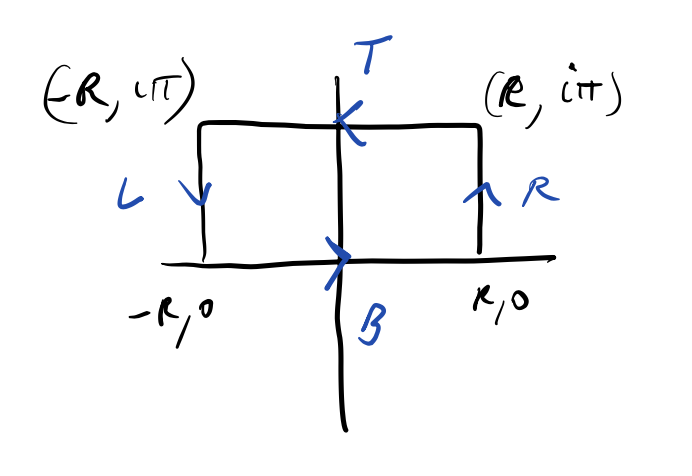
\includegraphics[width=0.65\textwidth]{contour1.png} % jpg/png/pdf/eps
\end{figure}
In the limit that we send $R\to\infty$ we see the $B$ is our integral of interest. We can see that
$$
T = \int_{R}^{-R}\frac{e^{ip(x+i\pi)}}{\cosh{(x+i\pi)}} = e^{-\pi p}\int_{-R}^{R}\frac{e^{ipx}}{\cosh{(x)}} = e^{-\pi p}B
$$
We can also see that $L$ and $R$ will go to zero in the limit
$$
\begin{aligned}
|R| = 	\left|\int_{0}^{\pi} \frac{e^{ip(R+iy)}}{\cosh(R+iy)}\, i\,dy\right|
	&\le \int_{0}^{\pi} \frac{|e^{ip(R+iy)}|}{|\cosh(R+iy)|}\,dy
	\le \int_{0}^{\pi} \frac{dy}{\sinh R}
	= \frac{\pi}{\sinh R}\xrightarrow{R\to\infty}0\\[4pt]
|L| = 	\left|\int_{\pi}^{0} \frac{e^{ip(-R+iy)}}{\cosh(-R+iy)}\, i\,dy\right|
	&\le \int_{0}^{\pi} \frac{|e^{ip(-R+iy)}|}{|\cosh(-R+iy)|}\,dy
	\le \int_{0}^{\pi} \frac{dy}{\sinh R}
	= \frac{\pi}{\sinh R}\xrightarrow{R\to\infty}0
\end{aligned}
$$
We conclude that 
$$
\tilde{f}_{3}(p) = \frac{2\pi e^{-\frac{\pi p}{2}}}{1+e^{-\pi p}}
$$
\item We see that $f_{4}(x) = e^{-x^{2}/2}-2x^{2}e^{-x^{2}/2}$. So
$$
\tilde{f}_{4}(p) = \mathcal{F}[e^{-x^{2}/2}]-2\mathcal{F}[x^{2}e^{-x^{2}/2}] = e^{-p^2/2}+2\partial_{p}^2e^{-p^2/2} =e^{-p^2/2}(2p^2-1)$$
\end{itemize}
} 
\begin{exercise}
	Define the Fourier transform for the function on a segment $x \in [0, L]$, vanishing at the boundaries, by
	\[
	f(x) = \sum_{k=1}^{\infty} \tilde{f}_k \sin\frac{\pi kx}{L}.
	\]
	Find the inverse transformation.
\end{exercise}



}
\lecture{7}{Properties of Fourier Transform Continued}
We continue our study of the properties of the fourier transform. We have  transformations for 3 different scenarios.
\begin{itemize}
\item$\mathbb{Z}/n\mathbb{Z}\leftrightarrow\mathbb{Z}/n\mathbb{Z},\quad \tilde{f}(k)=\frac{1}{\sqrt{N}}\sum_{n=1}^{N}e^{-\frac{2\pi i nx}{N}}f(n)$
\item $\mathbb{Z}\leftrightarrow S^{1},\quad \tilde{f}_{n} = \int_{0}^{2\pi}\frac{d\phi}{2\pi}e^{in\phi}f(\phi)$
\item $\mathbb{R}\leftrightarrow\mathbb{R}: \tilde{f}(p)\int_{-\infty}^{+\infty}dxe^{ipx}f(x)$
\end{itemize}
For now we will study the transform onto the circle, the second one. We have three goals. 
\begin{enumerate}
\item Find behavior of $\tilde{f}_{n}$
\item Show that the inverse transform is $f(\phi)=\sum_{n\in\mathbb{Z}}\tilde{f}_n e^{in\phi}$
\item Study the rate of convergence
\end{enumerate}
Let $f(\phi)\in C^{0}(S^{1})$ be a continuous function, even piecewise continuous is fine. What does this mean for $\tilde{f}_n$. First we need to define the scalar product on the circle.
\begin{align}
(f,g) = \int_{-\infty}^{\infty}f^{*}(\phi)g(\phi)\frac{d\phi}{2\pi}
\end{align}
Now we have the following lemma.
\begin{align}
	\sum_{n=-\infty}^{\infty}|\tilde{f}_{n}|^{2}<\infty
\end{align}
That is, the series of transformed values on the lattice space converges. So we are not going to get nonsense when we transform the function. We use the scalar product to define an orthogonal projection. 
\begin{align}
\tilde{f}_{n} = (e^{in\phi},f)
\end{align}
The complex exponentials form a basis for $S^{1}$ so we are just collapsing our function onto one of a continuous set of eigenvalues. Now we approximate $f$ by only summing over $2N+1$ weights\begin{align}
f(\phi) \approx f_{N}(\phi) = \sum_{k = -N}^{N} e^{ik\phi}\tilde{f}_{n} = \sum_{k = -N}^{N} e^{ik\phi}(e^{ik\phi},f) = (P_{N}f)(\phi)
\end{align}
We claim that $f_{N}(\phi) = (P_{N}f)(\phi)$ is a projector. That is $P_{N}^{2} = P_{N}$ We have
$$
P_{N}^{2}f = \sum_{k = -N}^{N} e^{ik\phi}(e^{ik\phi},\sum_{k^{\prime} = -N}^{N}e^{ik^{\prime}\phi}(e^{ik^{\prime}\phi},f)) = P_{N}^{2}f = \sum_{k = -N}^{N} e^{ik\phi}(\sum_{k^{\prime} = -N}^{N}\delta_{k,k^{\prime}}(e^{ik^{\prime}\phi},f)) = \sum_{k=-N}^{N}e^{ik\phi}(e^{ik\phi},f) = P_{N}f
$$
We also have two other properties.
\begin{itemize}
\item $(1-P_{N})^{2} = 1 -P_{N}$
\item $(P_{N}f,g) = (f,P_{N}g)$ (self-adjoint)
From properties of the inner product we have
$$
(f_{N}(\phi),f_{N}(\phi))\geq 0
$$
We expand the LHS to get
$$
(1-P_{N}f,(1-P_{N})f) = (f,f)-2(f,P_{N}f) +(P_{N}f,P_{N}f) = (f,f)-\sum(P_{N}f,P_{N}f) = (f,f) - \sum_{n=-N}^{N}|\tilde{f}_{n}|^{2}\geq 0
$$
\end{itemize}
So we have
$$
\sum_{n=-N}^{N}|\tilde{f}_{n}|^{2}\leq (f,f)
$$
Since the partial sums
\[
S_{N} = \sum_{n=-N}^{N} |\tilde{f}_{n}|^{2}
\]
satisfy \( 0 \le S_{N} \le (f,f) \) and increase monotonically with \( N \), 
by the Monotone Convergence Theorem the limit exists and is finite:
\[
\lim_{N \to \infty} S_{N} = \sum_{n=-\infty}^{\infty} |\tilde{f}_{n}|^{2} \le (f,f) < \infty.
\]
Hence
\[
\sum_{n=-\infty}^{\infty} |\tilde{f}_{n}|^{2} < \infty.
\]All the modes or weights must go to zero otherwise the sum will not converge.
Now let us consider the rate of convergence. If $f$ is differentiable and periodic, then
\begin{align}
	\widetilde{f'}_{n} 
	&= \int_{0}^{2\pi}\frac{d\phi}{2\pi}\, e^{-in\phi}f'(\phi)
	= \Big[\frac{e^{-in\phi}f(\phi)}{2\pi}\Big]_{0}^{2\pi}
	+ in\int_{0}^{2\pi}\frac{d\phi}{2\pi}\, e^{-in\phi}f(\phi)
	= in\,\tilde{f}_{n},
\end{align}
where the boundary term vanishes by periodicity. Hence
\[
\widetilde{f'}_{n} = in\,\tilde{f}_{n}.
\]
Applying the same reasoning repeatedly gives
\[
\widetilde{f^{(k)}}_{n} = (in)^{k}\tilde{f}_{n}.
\]
From this and the assumption that $f^{(k)} \in L^{2}(S^{1})$, it follows from Plancherel’s theorem that
\[
\sum_{n\in\mathbb{Z}} |\widetilde{f^{(k)}}_{n}|^{2} = 
\sum_{n\in\mathbb{Z}} |n|^{2k} |\tilde{f}_{n}|^{2} < \infty.
\]
Because this weighted series converges, its individual terms must tend to zero:
\[
|n|^{2k} |\tilde{f}_{n}|^{2} \longrightarrow 0 
\quad \text{as } |n| \to \infty.
\]
Hence there exists a constant $C > 0$ such that
\[
|\tilde{f}_{n}|^{2} \le \frac{C}{|n|^{2k}} 
\quad \Rightarrow \quad 
|\tilde{f}_{n}| \le \frac{\sqrt{C}}{|n|^{k}}.
\]
In big--O notation, we write this as
\[
|\tilde{f}_{n}| = O(|n|^{-k}) \qquad (|n| \to \infty)
\]

In words, the smoother the function $f$, the faster its Fourier coefficients decay.  
\begin{itemize}
	\item If $f$ is merely continuous, then $\tilde{f}_{n} \to 0$ (no specific rate).  
	\item If $f \in C^{1}$, then $\tilde{f}_{n} = O(1/n)$.  
	\item If $f \in C^{\infty}$, then $\tilde{f}_{n}$ decays faster than any power of $1/n$.  
	\item If $f$ is analytic, then $\tilde{f}_{n}$ decays exponentially, e.g.\ $|\tilde{f}_{n}| \sim e^{-|n|}$.  
\end{itemize}
So the less smooth the function is, the more fourier modes will be required to describe it well. Truncations of the modes for numerics and so on will be much better for very smooth functions. We have analagous results for the transfrom between $\mathbb{R}\leftrightarrow\mathbb{R}$. 
\begin{align*}
	\widetilde{f^{(k)}}(p) &= (ip)^{k}\tilde{f}(p), &
	\frac{d^{k}\tilde{f}}{dp^{k}}(p) &= (-i)^{k}\,\widetilde{x^{k}f(x)}(p), \\[4pt]
	x f(x) &\leftrightarrow i\,\frac{d\tilde{f}}{dp}, &
	f'(x) &\leftrightarrow (ip)\tilde{f}(p), \\[4pt]
	f^{(k)}\in L^{1}(\mathbb{R}) &\Rightarrow |\tilde{f}(p)|=O(|p|^{-k}), &
	f^{(k)}\in L^{2}(\mathbb{R}) &\Rightarrow \int |p|^{2k}|\tilde{f}(p)|^{2}dp<\infty, \\[4pt]
	f\text{ continuous} &\Rightarrow \tilde{f}(p)\text{ bounded, cont.}, &
	f\in C^{1} &\Rightarrow \tilde{f}(p)=O(1/p), \\[4pt]
	f\in C^{\infty} &\Rightarrow \tilde{f}(p)\text{ decays faster than any power}, &
	f\text{ analytic} &\Rightarrow \tilde{f}(p)\sim e^{-|p|}.
\end{align*}
Now consider the following example on $\mathbb{R}\leftrightarrow\mathbb{R}$.  We would like to transform
$$
\tilde{f}(p) = \frac{1}{p+i\gamma}
$$
back to position space. We will use the residue theorem, which Pavlo derives. But I skip the derivation. The transform is given by
$$
f(x) = \frac{1}{2\pi}\int_{-\infty}^{\infty}\frac{e^{ipx}}{p+i\gamma}dp
$$
\begin{figure}[H]
	\centering
	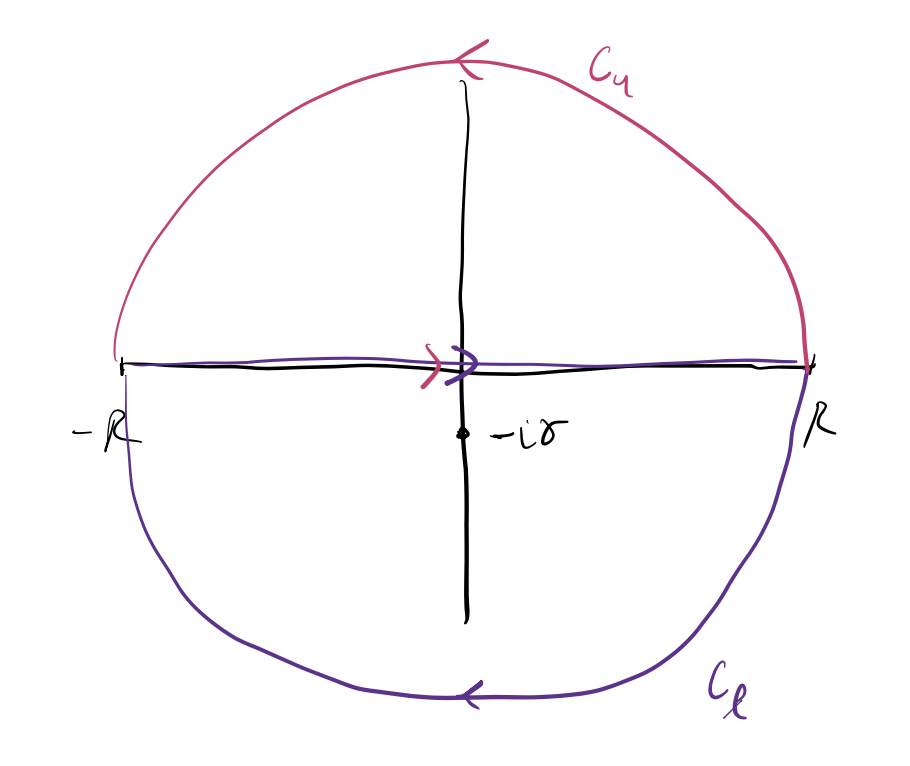
\includegraphics[width=0.45\textwidth]{contour4.png} % jpg/png/pdf/eps
\end{figure}
We will complexify momentum and use the residue theorem to calculate the integral.
$$
\lim_{R\to\infty}\frac{1}{2\pi}\oint \frac{e^{izx}}{z+i\gamma}dz = \frac{1}{2\pi}\lim_{R\to\infty}\big[\int_{-R}^{R}\frac{e^{ipx}}{p+i\gamma}dp + \int_{C}\frac{e^{izx}}{z+i\gamma}\big]
$$
The first integral is the target integral we wish to find. substituting $z = Re^{i\theta}$ in the second integral we have
$$
\int_{C}\frac{e^{izx}}{z+i\gamma} = \int_{0}^{\pi}\frac{iRe^{i(\theta+R\cos{\theta})}e^{-R\sin{\theta}x}}{Re^{i\theta}+i\gamma}d\theta
$$
We can bound the argument by 
$$
\Big|\frac{iRe^{i(\theta+R\cos{\theta})}e^{-Rx\sin{\theta}}}{Re^{i\theta}+i\gamma}\Big|\leq \frac{|Re^{-Rx\sin{\theta}}|}{|R|-|\gamma|}  \xrightarrow{R\to\infty} 0
$$
when $x>0$ and $\sin\theta > 0$ or $x<0$ and $\sin\theta < 0$. We choose our contours accordingly to get 
\[
f(x) =
\begin{cases}
	0, & x > 0, \\[6pt]
	-i\,e^{\gamma x}, & x < 0.
\end{cases}
\] 
This example illustrates the general relationships we established earlier between smoothness, differentiability, and the decay of Fourier transforms.

\begin{itemize}
	\item The position--space function
	\[
	f(x) =
	\begin{cases}
		0, & x > 0, \\[4pt]
		-i\,e^{\gamma x}, & x < 0,
	\end{cases} = -i\Theta(-x)e^{\gamma x}
	\]
	is continuous but not differentiable at $x=0$. 
	Hence, by the earlier results, we should not expect $\tilde{f}(p)$ to decay faster than $O(1/p)$, 
	which is consistent with
	\[
	\tilde{f}(p) = \frac{1}{p+i\gamma}.
	\]
	Indeed, $|\tilde{f}(p)| \sim 1/|p|$ for large $|p|$.
	
	\item The discontinuity in the derivative at $x=0$ produces only a \emph{power--law decay} in $\tilde{f}(p)$,
	whereas a smooth or analytic $f(x)$ would yield much faster decay.
	
	\item The parameter $\gamma>0$ controls the exponential decay rate of $f(x)$ for $x<0$:
	\[
	|f(x)| = e^{\gamma x} = e^{-|x|/\xi},
	\qquad \text{with decay length } \xi = \frac{1}{\gamma}.
	\]
	Increasing $\gamma$ makes $f(x)$ more localized in $x$, 
	and correspondingly $\tilde{f}(p)$ becomes broader in momentum space.
	This again reflects the uncertainty--like tradeoff between localization and spectral spread.
	
	\item Thus this simple example encapsulates two of the general properties discussed earlier:
	\begin{enumerate}
		\item Less smoothness in $x$ $\Rightarrow$ slower decay of $\tilde{f}(p)$,
		\item Faster spatial decay (larger $\gamma$) $\Rightarrow$ broader Fourier distribution.
	\end{enumerate}
\end{itemize}
\problems{
\begin{exercise}
	Find the Fourier transform of the function
	\[
	f(x) = \frac{1}{x^2 + 1}
	\]
	on $\mathbb{R}$.
\end{exercise}
\solution{
We have
$$
\tilde{f}(p) = \int_{-\infty}^{\infty} \frac{e^{ipx}}{x^{2}+1}dx
$$
which has two poles in the complex plane. So we complexify to get
$$
\oint \frac{e^{ipz}}{z^{2}+1} = \oint\frac{e^{ipx}e^{-py}}{z^{2}+1}
$$
with $z=x+iy$. We use the following contour
\begin{figure}[H]
	\centering
	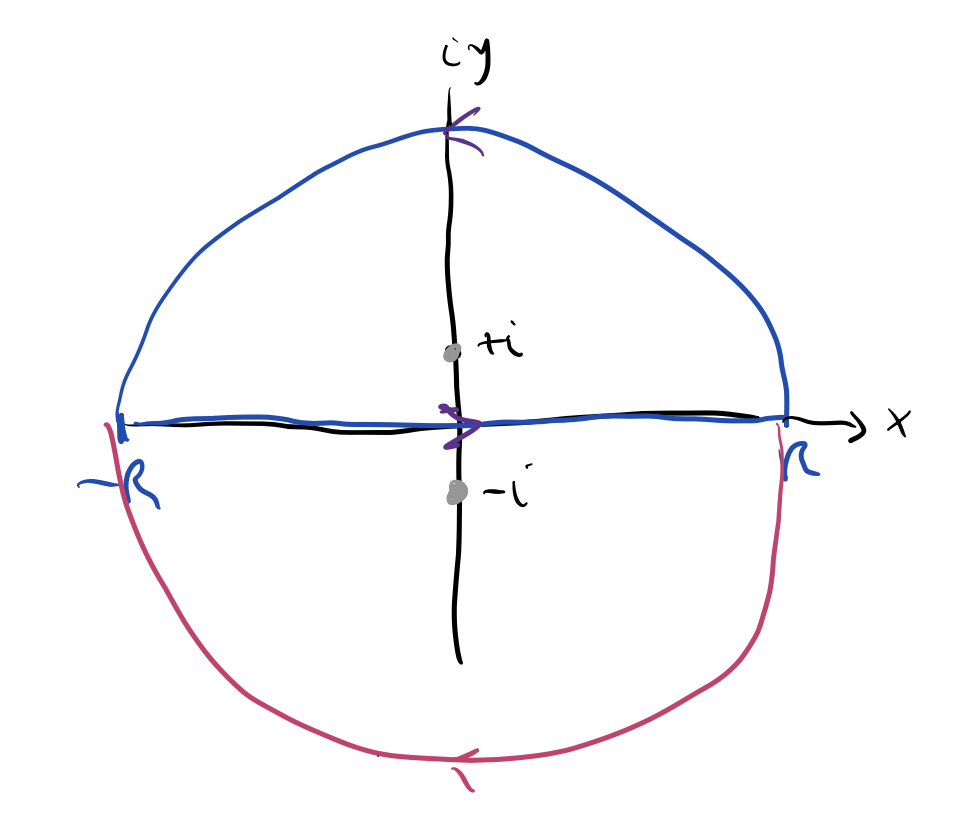
\includegraphics[width=0.65\textwidth]{contour2.png} % jpg/png/pdf/eps
\end{figure}
}
For $p>0$ we must use the upper contour where $y>0$. For $p<0$ we must use the lower contour where $y<0$. Using spherical coordinates $z = Re^{i\theta}$ we have the integral over the upper arc is
$$
\int_{0}^{\pi}\frac{e^{ipRe^{i\theta}}}{R^{2}e^{i2\theta}+1}iRe^{i\theta}d\theta
$$
One can show that the absolute value of the integrand is bounded by
$$
|\frac{Re^{-pR}}{R^{2}-1}|\xrightarrow{R\to\infty} 0
$$
So this integral vanishes. We calculate the residue to be $\pi e^{-p}$ for $p>0$. A similar argument goes for the lower contour and we find that the lower contour integral for $p<0$ gives the residue $\pi e^{p}$. Our final transformed function is 
$$
\tilde{f}(p) = \pi e^{-|p|}
$$
\begin{exercise}
	Find the Fourier transform of the function
	\[
	f(x) = \frac{\sin x}{x^2 + 1}
	\]
	on $\mathbb{R}$.
\end{exercise}
\solution{
We would like to find
$$
\int_{-\infty}^{\infty}\frac{\sin(x)e^{ipx}}{x^{2}+1}dx
$$
We have the same poles as in teh previous problem so we use the same contour. Using the exponential definiton of $\sin{(x)}$ we get
$$
\tilde{f}(p)=\frac{1}{2i}\big[\int_{-\infty}^{\infty}\frac{e^{i(p+1)}}{x^{2}+1}-\int_{-\infty}^{\infty}\frac{e^{i(p-1)}}{x^{2}+1}\big]
$$
But this if we complexify this is exactly the same contour integral as the previous question but with $p\to\pm1$. Using the previous result we get
$$
\tilde{f}(p) = \frac{i\pi}{2}\big[e^{-|p-1|}-e^{-|p+1|}\big]
$$
}
\begin{exercise}
	Find the Fourier transform of the function
	\[
	f(x) = \frac{\sin x}{x}
	\]
	on $\mathbb{R}$.
\end{exercise}
}
\solution{
Using the exponetial definition of the sine function we have
$$
\tilde{f}(p)\frac{1}{2i}\big[\int_{-\infty}^{\infty}\frac{e^{i(p+1)x}}{x}-[\int_{-\infty}^{\infty}\frac{e^{i(p-1)x}}{x}\big]
$$
When we complexify these integrals we will have two choices of contour.
\begin{figure}[H]
	\centering
	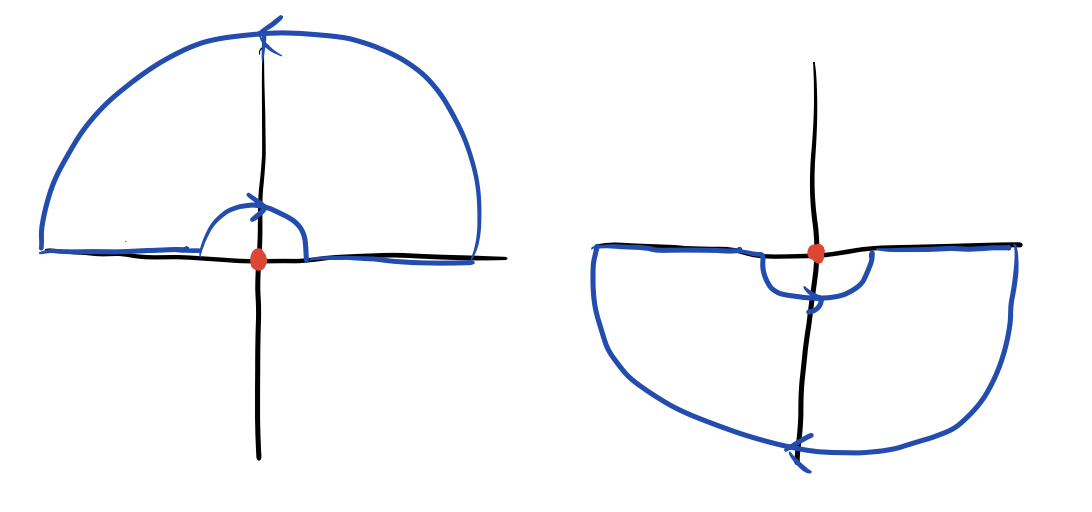
\includegraphics[width=0.65\textwidth]{contour3.png} % jpg/png/pdf/eps
\end{figure}

In both cases 
$$
\lim_{R\to\infty}\lim_{\epsilon\to0}\oint \frac{\sin{(z)e^{ipz}}}{z}dz = 0
$$
For $p+1>0$ we use the upper contour for the first integral and for $p+1<0$ we use the lower contour. For $p-1>0$ we use the upper arc for the second integral and for $p-1<0$ we use the lower contour. In this way taking the limit of $R\to\infty$ will cause the large arc to vanish. Since the entire contour is $0$ that means our targe integral is the negative of the arc of radius $\epsilon$ around the pole. Setting up the integral on the small arc and taking $\epsilon\to 0$ gives trivial integrals. 
We find that we have
\[
\tilde{f}(p) =
\begin{cases}
	\dfrac{\pi}{2}, & p > -1, \\[6pt]
	-\dfrac{\pi}{2}, & p \le -1
\end{cases}
\quad - \quad
\begin{cases}
	\dfrac{\pi}{2}, & p > 1, \\[6pt]
	-\dfrac{\pi}{2}, & p \le 1
\end{cases}
\]
This is just a rectangle of height $\pi$ from $x=-1$ to $x = 1$ and $0$ everywhere else.
}
\lecture{8}{Finishing Fourier Transform on a Circle and Intro to Generalized Functions}
We continue studying properties of Fourier transforms. In the last lecture we ended with the result
$$
\frac{1}{p+i\gamma},\ \gamma >0 \leftrightarrow - i\Theta_{H}(-x)e^{\gamma x}
$$
We arrived at this result via the contour integral. The rate of decay depends on the singularity in momentum space. Using the fact that
$$
\frac{1}{p-i\gamma},\ \gamma>0 \leftrightarrow i\Theta_{H}(x)e^{-\gamma x}
$$
We can piece these results together to get
$$
\frac{1}{p+i\gamma} - \frac{1}{p-i\gamma},\ \gamma>0 \leftrightarrow -ie^{-\gamma |x|}
$$
Condensing the lefthand side gives us
$$
-\frac{2i\gamma}{p^{2}+\gamma^{2}}
$$
Using the fourier transform we get the following integral identity
$$
\int_{-\infty}^{\infty}\frac{2}{\pi}\frac{\gamma e^{ipx}}{p^{2}+\gamma^{2}} dp= e^{-\gamma|x|}
$$
At $x=0$ we get
$$
\int_{-\infty}^{\infty}\frac{2}{\pi}\frac{\gamma}{p^{2}+\gamma^{2}} = 1
$$
We can use this in our computations. Now we turn to finding the inverse fourier transform on $S^{1}$. Previously we had
$$
\tilde{f}_{n} = \int_{0}^{2\pi}\frac{d\phi}{2\pi}e^{-in\phi}f(\phi)
$$
We proved with a lemma that 
$$
f(\phi)=\sum_{n\in\mathbb{Z}}\tilde{f}_{n}e^{in\phi}
$$
We omit the detailed proof of convergence, but now we can use this inverse transform. Another important feature of a fourier series of a discontinuous function is that it
does not converge pointwise at the jump: it exhibits oscillations known as the Gibbs Phenomenon. 
These oscillations arise from the sinc--like kernel $\sin x/x$ that governs Fourier reconstruction. 
The integral
\[
I = \int_{-\infty}^{\infty}\frac{\sin x}{x}\,dx = \pi
\]
illustrates the normalization of the sinc kernel and shows how Fourier approximations 
reproduce the correct average value across a discontinuity, even though they fail to converge 
pointwise. The sinc function effectively approximates the Dirac delta, and the Gibbs phenomenon 
expresses the limitation of representing discontinuous functions with smooth Fourier modes. 
This naturally motivates the theory of \textit{generalized functions}, which extends the notion of 
a function so that differentiation and Fourier transformation remain well defined even for 
discontinuous or non--integrable cases. Within this framework the Dirac delta $\delta(x)$ and its 
derivatives are rigorously defined, identities such as $\frac{d\Theta_{H}}{dx}=\delta(x)$ hold, and 
Fourier transforms of singular objects like $1$ or $1/(p+i\epsilon)$ acquire precise meaning. 
Distributions thus provide a consistent language for handling discontinuities, singularities, and 
limiting prescriptions that frequently arise in physics.
Here are some common results.
\begin{align*}
	\delta(ax) &= \frac{1}{|a|}\,\delta(x), &
	x\,\delta(x) &= 0, &
	\int_{-\infty}^{\infty}\delta(x)\,dx &= 1, \\[4pt]
	\frac{d\Theta_{H}}{dx} &= \delta(x), &
	\frac{d\,\operatorname{sgn}(x)}{dx} &= 2\delta(x), &
	\frac{d\,\delta(x)}{dx} &= -\delta'(x), \\[4pt]
	\mathcal{F}\{\delta(x)\} &= 1, &
	\mathcal{F}\{1\} &= 2\pi\delta(p), &
	\mathcal{F}\{\Theta_{H}(x)\} &= \pi\delta(p) + \frac{i}{p}, \\[4pt]
	\mathcal{F}\{\operatorname{sgn}(x)\} &= \frac{2}{ip}, &
	\mathcal{F}\{x f(x)\} &= i\,\frac{d\tilde{f}}{dp}, &
	\mathcal{F}\{f'(x)\} &= (ip)\tilde{f}(p).
\end{align*}


\problems{
\begin{exercise}
	Find the Fourier transform of the function
	\[
	f(x) = \frac{1}{e^{2\pi i x} - \frac{1}{2}}
	\]
	on a circle $x \sim x + 1$.
\end{exercise}
\solution{
When we transform functions on a circle we go between $\mathbb{Z}\leftrightarrow S^{1}$. The weights are given by
$$
\tilde{f}_{n}= \int_{0}^{1}\frac{dx}{2\pi}e^{-2\pi inx}\frac{1}{e^{2\pi i x}-\frac{1}{2}}
$$
If we substitute $z=e^{2\pi ix}$ we get the following contour integral
$$
\frac{1}{2\pi i}\oint_{|z|=1}\frac{z^{-n-1}}{z-\frac{1}{2}}
$$
We see there is a pole inside the contour at $z=\frac{1}{2}$. Calculating the residue gives us the weights 
$$
\tilde{f}_{n} = 2^{n+1}$$
\textcolor{red}{not defined for all n}
}
\begin{exercise}
	Find the Fourier transform of the function
	\[
	f(x) = \frac{1}{\cos(2\pi x) - \cosh(2\pi a)}
	\]
	on a circle $x \sim x + 1$.
\end{exercise}
\solution{
We would like to find
$$
\tilde{f}_{n}= \int_{0}^{1}\frac{-2e^{2\pi i nx}}{e^{i2\pi x}+e^{-i2\pi x}-2\cosh{(2\pi a)}}dx = \frac{1}{\pi i}\oint_{|z|=1}\frac{z^{-n}}{z^{2}-(e^{-2\pi a}+ e^{2\pi a})z+1}dz
$$
where we used the exponential definitions of $\cos$ and $\cosh$, compexified and substituted $z= e^{i2\pi x}$. We see the denominator factors into $(z-e^{2\pi a})(z-e^{-2\pi a})$. We are assuming $a\in \mathbb{R}$ and $a>0$ so $z = e^{2\pi a}$ is outside the contour.
Calculating the residue and simplifying gives us 
$$
\tilde{f}_{n} = \frac{e^{-2\pi a n}}{\sinh{(2\pi a)}}
$$
\textcolor{red}{not defined for all n}
}
\begin{exercise}
	Compute the Fourier transforms of the following functions on a circle $\varphi \in [0, 2\pi)$:
	\[
	f_1(\varphi) = \varphi, \qquad f_2(\varphi) = |\pi - \varphi|.
	\]
	For $f_1$, determine the asymptotic behavior of the coefficients at large $n$.  
	For $f_2$, compute $f_2(0)$ and compare it with its Fourier series at this point. Does it yield any non-trivial identity?
\end{exercise}
\begin{exercise}
	Compute the Fourier transform of $\operatorname{v.p.}\frac{1}{\omega}$, then check that the inverse Fourier transform recovers the initial (generalized) function.
\end{exercise}
\lecture{9}{Generalized Functions and Weak Form of the Wave Equation}
}
Now we return to our transforms $f(x)\leftrightarrow\tilde{f}(p)$ and consider \textit{generalized functions}. 
These are continuous linear functionals acting on the space of smooth test functions 
$C^{\infty}(\mathbb{R})$, or more generally on $C^{\infty}(\mathbb{R}/S^{1}/\mathbb{R}^{n},\mathbb{C})$. 
A sequence of ordinary functions $\{f_{n}\}$ is said to converge \emph{weakly} to a generalized function $f$ 
if for every test function $\varphi$ we have
\[
f_{n} \to f_{\text{gen}} 
\quad \text{iff} \quad 
(f_{n},\varphi) \;\longrightarrow\; (f,\varphi),
\qquad 
\forall\,\varphi \in C^{\infty}(\mathbb{R}/S^{1}/\mathbb{R}^{n}...).
\]
Here $(f,\varphi)$ denotes the pairing or dual action, typically written as
\[
(f,\varphi) = \int f(x)\,\varphi(x)\,dx,
\]
whenever the integral exists.  
This defines convergence in the weak or distributional sense, 
and allows us to treat limits of oscillatory or singular sequences—such as those arising in Fourier analysis—
as well-defined generalized functions.
A family of ordinary functions $\{\delta_{\epsilon}(x)\}_{\epsilon>0}$ is called a 
\textit{delta sequence} if
\[
\lim_{\epsilon\to 0^{+}} \int_{-\infty}^{\infty} \delta_{\epsilon}(x)\,\varphi(x)\,dx 
= \varphi(0),
\qquad \forall\,\varphi\in C^{\infty}_{c}(\mathbb{R}).
\]
That is, $\delta_{\epsilon}\to\delta$ in the weak (distributional) sense.  
Typical examples include
\[
\delta_{\epsilon}(x)
= \frac{1}{\sqrt{\pi}\epsilon}e^{-(x/\epsilon)^{2}}, 
\qquad
\delta_{\epsilon}(x)
= \frac{1}{\pi}\frac{\epsilon}{x^{2}+\epsilon^{2}}, 
\qquad
\delta_{\epsilon}(x)
= \frac{\sin(x/\epsilon)}{\pi x}.
\]
Each of these satisfies the normalization condition
\[
\int_{-\infty}^{\infty}\delta_{\epsilon}(x)\,dx = 1,
\]
and becomes increasingly localized around $x=0$ as $\epsilon\to 0$. Let us return to the solution of the wave equation we found on $\mathbb{R}$, wo se can see an example of these generalized functions. For the equation $u_{xx}-u_{tt} = 0$ we had the solution  $u(x,t) = \frac{1}{2}(u_{0}(x-t)+u_{0}(x+t))$
\begin{figure}[H]
	\centering
	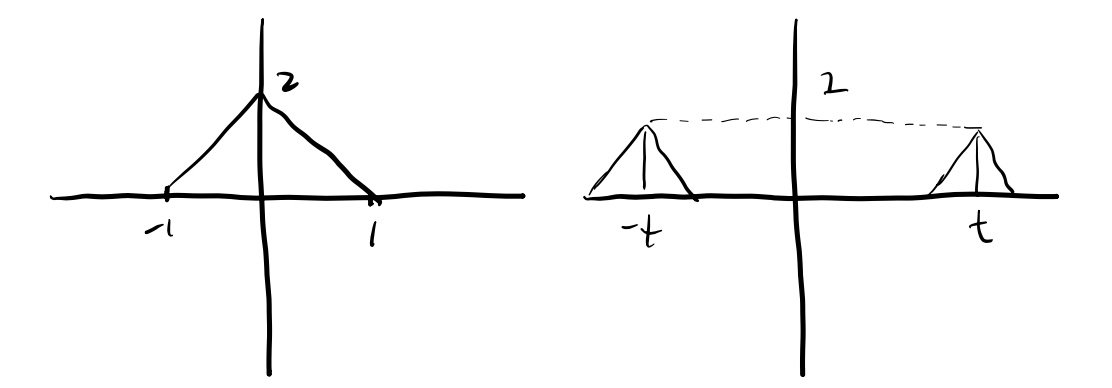
\includegraphics[width=0.45\textwidth]{wave1.png} % jpg/png/pdf/eps
\end{figure}
Now let us consider the derivatives. The first derivative is given by
\begin{figure}[H]
	\centering
	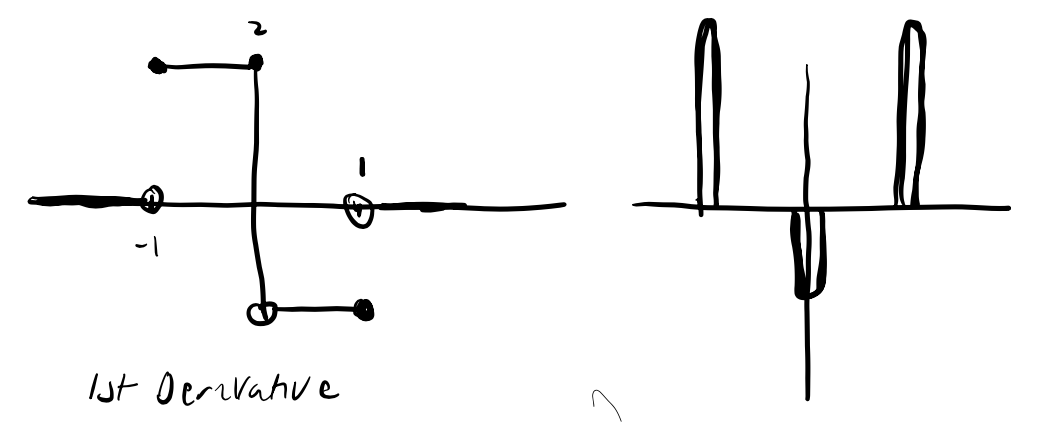
\includegraphics[width=0.45\textwidth]{derivatives.png} % jpg/png/pdf/eps
\end{figure}
We see that the colloquial  second derivative does not exists due to the discontinuities. But we still have an integrable function with $u_{xx}(0,x) = \delta(x-1)-2\delta(x)-\delta(x+1)$. To make this rigorous we must introduce the weak form of an equation. For our equation $u_{tt}-u_{xx} = f$ we have
$$
(u_{tt}-u_{xx},\varphi) = (f,\varphi)
$$
From this we have
$$
0 = \int_{-\infty}^{\infty}dx\int_{-\infty}^{\infty}dt\,(u_{tt}-u_{xx}-f)\varphi 
= (u,\varphi_{tt} - \varphi_{xx})-(f,\varphi) -(u_{0}(x),\varphi_{t}(0,x)) +(u_{1}(x),\varphi(0,x))
$$
which is the weak form of the wave equation and should hold for all arbitrary test functions $\varphi\in C_{c}^{\infty}(\mathbb{R})$. We have used integration by parts and the fact that $\varphi$ is compactly supported on $\mathbb{R}$ to remove boundary terms. Its called the weak form because our restrictions are much less strict. We only require continuity and not differentiability. We don't prove it but if the weak form is satisfied and $u\in C^{2}(\mathbb{R})$, then the original form of the wave equation is also satisfied. In this weak form our previous derivation with delta functions is also satisfied. Recall that we derived that any function $u = F(t - x)$ satisfies the $1+1$ wave equation.
\[
(F(t-x),\varphi_{tt}-\varphi_{xx}) = 
\int_{-\infty}^{\infty}\!dx \int_{-\infty}^{\infty}\!dt\,
F(t-x)\,(\varphi_{tt}-\varphi_{xx}).
\]
To make this computation more transparent, we introduce the light-cone variables
\[
a = t - x, \qquad b = t + x,
\]
so that
\[
t = \frac{a + b}{2}, \qquad x = \frac{b - a}{2}, \qquad
dt\,dx = \frac{1}{2}\, da\, db.
\]
In these variables the derivatives transform as
\[
\partial_t = \partial_a + \partial_b, \qquad
\partial_x = -\partial_a + \partial_b.
\]
Hence
\[
\partial_{tt} - \partial_{xx}
= (\partial_a + \partial_b)^2 - (-\partial_a + \partial_b)^2
= 4\,\partial_{ab}.
\]
Substituting into the integral, we obtain
\[
(F(t-x),\varphi_{tt}-\varphi_{xx})
= \int_{-\infty}^{\infty}\!dx \int_{-\infty}^{\infty}\!dt\,
F(t-x)\,(\varphi_{tt}-\varphi_{xx})
= 2\int_{-\infty}^{\infty}\!da \int_{-\infty}^{\infty}\!db\,
F(a)\, \partial_{ab}\varphi(a,b),
\]
where we used $dt\,dx = \frac{1}{2}\,da\,db$.

Now, since $\varphi(a,b)$ is a smooth test function with compact support,
we can integrate by parts in $b$:
\[
\int_{-\infty}^{\infty} \partial_{ab}\varphi(a,b)\, db
= \big[\partial_a\varphi(a,b)\big]_{b=-\infty}^{\infty} = 0.
\]
Thus the entire integral vanishes:
\[
(F(t-x),\varphi_{tt}-\varphi_{xx}) = 0.
\]

Therefore, $u(t,x) = F(t-x)$ satisfies
\[
(u_{tt}-u_{xx}, \varphi) = 0 \qquad \forall\, \varphi \in C_c^\infty(\mathbb{R}^{1+1}),
\]
which shows that $u = F(t-x)$ is a weak solution of the homogeneous $1+1$ wave equation.
The same computation holds for $u(t,x) = G(t+x)$ as well.
\newline

The weak (or distributional) form of a partial differential equation offers several important advantages. 
It allows us to define solutions even when classical derivatives do not exist, such as in problems involving 
discontinuities or singularities, by interpreting derivatives in the sense of distributions. 
This means we can work with functions that are merely integrable---often only in 
$L^1_{\text{loc}}$ or $L^2_{\text{loc}}$---rather than requiring them to be twice continuously differentiable. 
Boundary and initial conditions arise naturally through integration by parts, providing a rigorous way 
to handle them even for irregular domains or data. 
The weak formulation also forms the mathematical foundation of numerical methods like the finite element method, 
which approximate the PDE on finite-dimensional spaces of test functions. 
Moreover, it accommodates generalized functions such as delta distributions, allowing us to model point sources 
and impulses directly. 
Finally, weak solutions often exist and are unique even when classical solutions break down, 
making the weak form both a theoretical generalization and a practical framework for solving real-world PDEs.
\newline

Let us now use this to solve the wave equation with a point source.
$$
u_{tt}-u_{xx}=\delta(t)\delta(x) \Rightarrow (u,\varphi_{tt}-\varphi_{xx}) = (\delta(t)\delta(x),\varphi) = \varphi(0,0)
$$
We switch to the coordinates $\xi = x+t$ and $\eta = x-t$, so we get $\partial_{x} = \partial_{\xi} + \partial_{\eta}$ and $\partial_{t} = \partial_{\xi}-\partial_{\eta}$
or $\partial_{\xi} = \frac{1}{2}(\partial_{x}+\partial_{t})$ and $\partial_{\eta} = \frac{1}{2}(\partial_{x}-\partial_{t})$.
With these coordinates we have
$$
(u,\varphi_{\xi\eta}) = \frac{1}{2}\varphi(0,0)
$$
Let us transform back to the original form to get the solution.
$$
(u_{\xi\eta},\varphi) = \frac{1}{2}\varphi(0,0) \Rightarrow u_{\xi\eta} = \frac{1}{2}\delta(\xi)\delta(\eta)
$$
so $u = \delta(\xi)\delta(\eta)$. Let us use this strategy of transforming to the weak form to solve a simpler equation.
$$
u^{\prime}(x) = \delta(x)\Rightarrow -(u,\varphi^{\prime}) = \varphi(0)
$$
Since this should hold for any test function, we can use this to our advantage. We want to show this solution is a constant everywhere except 0. We will choose the test functions that are infinitely differentiable everywhere that are only non-zero in a small interval $[y-\epsilon,y+\epsilon]$
\begin{figure}[H]
	\centering
	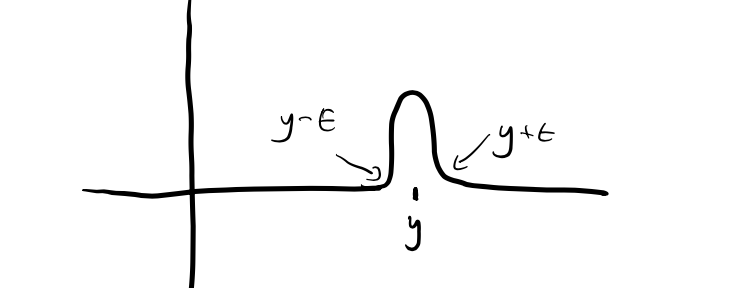
\includegraphics[width=0.45\textwidth]{compactsupport.png} % jpg/png/pdf/eps
\end{figure}
Thus we have
$$
-\int_{y-\epsilon}^{y+\epsilon}u\varphi^{\prime}dx = 0 = u^{\prime}
$$
Now lets see what happens at $x=0$. We can choose a test function 
$$
u = 
\begin{cases}
	u_{-}(x),\quad x<0 \\
	u_{+}(x),\quad  x>0
\end{cases}
$$
Now we have
$$
-\int_{-\infty}^{\infty}u(x)\varphi^{\prime}(x) = -\int_{0^{+}}^{\infty}u_{+}(x)\varphi^{\prime}(x)dx - \int_{-\infty}^{0^{-}}u_{-}(x)\varphi^{\prime}(x)dx = \big(u_{+}-u_{-}\big)\varphi(0) = \varphi(0)
$$
But $\varphi(0+\epsilon) =\varphi(0-\epsilon) = \varphi(0)$ because $\varphi$ is smooth and therefore continuous across $x=0$ (and compactly supported, so it vanishes at $\pm\infty$). So we get
$$
(u_{+}(x)-u_{-}(x)) = 1
$$
From this we can conclude the identity
$$
u(x) = C + \Theta_{H}(x),
$$
where $\Theta_{H}(x)$ is the Heaviside step function satisfying $\Theta_{H}'(x)=\delta(x)$.
\begin{center}
\textcolor{red}{skipped last 8 minutes of lecture video}	
\end{center}
\lecture{10}{Applications of Fourier Transform To Solving PDEs}
\begin{center}
\textcolor{red}{extremely useful, review lecture video}
\end{center}




\newpage
\lecture{X}{More Problems}
\problems{

\begin{exercise}
	Solve the equation
	\[
	u''(t) + \omega^2 u(t) = f(t), \quad u(0) = u_0, \quad u'(0) = u_1.
	\]
\end{exercise}










\begin{exercise}
	Find the plane wave solution of Maxwell’s equations.
\end{exercise}




\begin{exercise}
	Solve the following equation:
	\[
	u''(t) + \mu^2 u(t) = \theta_H(t)\sin\Omega t, \quad u(0) = u'(0) = 0.
	\]
	What is the difference between the cases $\Omega^2 \neq \mu^2$ and $\Omega^2 = \mu^2$?
\end{exercise}

\begin{exercise}
	Solve the heat equation on the real line:
	\[
	u_t(t, x) = \Delta u(t, x), \quad u(0, x) = \theta_H(x).
	\]
	How smooth is $u(t, x)$ for $t > 0$?
\end{exercise}



\begin{exercise}
	Solve Laplace’s equation $u_{z\bar{z}} = 0$ in the unit disk $|z| \le 1$ with the following boundary conditions:
	\[
	u(e^{i\varphi}) =
	\begin{cases}
		\cos \varphi, \\
		1, & \varphi \in (0, \pi),\\
		-1, & \varphi \in (\pi, 2\pi).
	\end{cases}
	\]
\end{exercise}

\begin{exercise}
	Find the Green function of the Laplace equation in the domain
	\[
	D = \{z \mid \Im z \in [0, \pi], \; \Re z \in [0, \infty)\}
	\]
	with boundary conditions $G(z, z_0) = 0$ for $z \in \partial D$ and $G(z, z_0) \to 0$ as $\Re z \to \infty$.
	
	\textit{Idea 1:} first solve in the infinite strip, then add image charge.  
	\textit{Idea 2:} use conformal map $w(z) = \cosh z$.
\end{exercise}

\begin{exercise}
	Solve Laplace’s equation $u_{z\bar{z}} = 0$ in the domain
	\[
	D = \{z \mid \Re z \ge 0, |z - 1| \le a\}
	\]
	with boundary conditions:
	\[
	u = 0, \; z \in i\mathbb{R}, \quad
	u = u_0, \; |z - 1| = a, \quad
	u \to 0 \text{ as } z \to +\infty.
	\]
\end{exercise}

\begin{exercise}
	Solve the 3D Laplace equation $\Delta u = 0$ in the domain
	\[
	D = \{(r, \theta, \varphi) \mid r > R\}
	\]
	with boundary conditions
	\[
	u(R, \theta, \varphi) = \cos^2\theta, \qquad \lim_{r \to \infty} u(r, \theta, \varphi) = 0.
	\]
\end{exercise}

\begin{exercise}
	Find all solutions of Laplace’s equation $\Delta u(x, y, z) = 0$ which are not more than quadratic in $x, y, z$.  
	Expand them in spherical harmonics.
\end{exercise}

\begin{exercise}
	Compute the scalar product between associated Legendre polynomials:
	\[
	\int_{-1}^{1} P_l^m(x) P_k^m(x)\,dx.
	\]
	Definition:
	\[
	P_l^m(x) = (-1)^m (1 - x^2)^{m/2} \frac{d^m}{dx^m} P_l(x), \quad
	P_l(x) = \frac{1}{2^l l!} \frac{d^l}{dx^l}(x^2 - 1)^l.
	\]
\end{exercise}

\begin{exercise}
	Find the Fourier expansion of the plane wave:
	\[
	e^{ikr\sin\varphi} = \sum_{n\in\mathbb{Z}} c_n(r)e^{in\varphi}.
	\]
\end{exercise}
}


\begin{exercise}
	Find the Fourier transform of $\frac{1}{\cosh x}$.
	
	\textit{Hints:}
	\begin{itemize}
		\item Consider the difference of the two integrals over $\mathbb{R}$ and over $\mathbb{R} + 2\pi i$: first compare it with the original integral, then compute by residues.
		\item Alternatively, close the contour and compute it as a sum of residues.
	\end{itemize}
\end{exercise}

\begin{exercise}
	Solve the equation
	\[
	u_{tt} - u_{xx} = f(t, x), \quad u_t(0, x) = 0, \quad u(0, x) = 0,
	\]
	where
	\[
	f(t, x) = |1 - |x|| \, \theta_H(1 - |x|)\theta_H(t(1 - t)).
	\]
	Plot this solution, e.g. for $t = 10$.
\end{exercise}



\begin{exercise}
	Solve the equation
	\[
	u_t - u_{xx} = 0, \qquad u(0, x) = \sin x.
	\]
\end{exercise}

\begin{exercise}
	Solve the equation
	\[
	u_t - u_{xx} = 0, \quad x \ge 0, \quad |u(-\infty, x)| < \infty, \; |u(t, +\infty)| < \infty, \quad u(t, 0) = \sin t.
	\]
\end{exercise}


\begin{exercise}
	Find a formula for $P^1_{f(x)}$, analogous to
	\[
	\delta(f(x)) = \sum_{f(x_n) = 0} \frac{1}{|f'(x_n)|}\delta(x - x_n).
	\]
\end{exercise}

\begin{exercise}
	Solve the equation
	\[
	u_t(t, \vec{r}) - \Delta u(t, \vec{r}) = 0, \quad \vec{r} \in \mathbb{R}^d, \quad u(0, \vec{r}) = \vec{r}\, e^{-(\vec{r} - \vec{r}_0)^2}.
	\]
\end{exercise}

\begin{exercise}
	Solve the equation
	\[
	\Delta u(x, y) = 0, \quad x^2 + y^2 \le 1, \quad u(\cos \varphi, \sin \varphi) = \sin 2\varphi.
	\]
\end{exercise}

\begin{exercise}
	Solve the equation
	\[
	\partial_t u(t, x) - u_{xx}(t, x) = \sin x \sin t, \quad u(0, x) = 0,
	\]
	in the limit $t \to \infty$.
\end{exercise}

\begin{exercise}
	Solve the equation
	\[
	\Delta u(x, y, z) = 0, \quad x^2 + y^2 + z^2 \le 1, \quad u(\sin\theta\cos\varphi, \sin\theta\sin\varphi, \cos\theta) = \cos 2\theta.
	\]
\end{exercise}

\begin{exercise}
	Solve the equation
	\[
	\Delta u(x, y) = \delta(x - x_0)\delta(y - y_0),
	\]
	in the domain $\arg(x + iy) \in (0, \pi/3)$ with boundary conditions
	\[
	u(r\cos \tfrac{\pi}{3}, r\sin \tfrac{\pi}{3}) = u(r, 0) = 0.
	\]
\end{exercise}

\begin{exercise}
	Expand each component of the vector
	\[
	(\sin\theta\cos\varphi, \sin\theta\sin\varphi, \cos\theta)P_1(\cos\theta)
	\]
	in the basis of spherical harmonics.
\end{exercise}

\begin{exercise}
	Find solutions of the Sturm–Liouville problem
	\[
	u''(x) = -\lambda u(x), \quad u(0) = 0, \quad u'(1) = 0.
	\]
	Check that the corresponding functions $u_n(x)$ form a complete system.
\end{exercise}

\begin{exercise}
	Find the radially symmetric solution of the Helmholtz equation
	\[
	\Delta u(r) + u(r) = 0,
	\]
	regular at $r = 0$, in two and three dimensions.
\end{exercise}
\begin{exercise}
	Solve the wave equation:
	\[
	\begin{cases}
		u_{tt} - u_{xx} - u_{yy} = (\theta_H(t - 1) - \theta_H(t - 2)) \delta(x)\delta(y), & u(0, x, y) = u_t(0, x, y) = 0, \\
		u_{tt} - u_{xx} - u_{yy} - u_{zz} = (\theta_H(t - 1) - \theta_H(t - 2)) \delta(x)\delta(y)\delta(z), & u(0, x, y, z) = u_t(0, x, y, z) = 0.
	\end{cases}
	\]
\end{exercise}
\begin{exercise}
	Solve the equation
	\[
	u_{tt} - u_{xx} - u_{yy} = \delta(x)\delta(y)\theta_H(t(1 - t)), \quad t > 0, \quad u(0, x, y) = u_t(0, x, y) = 0.
	\]
\end{exercise}
\begin{exercise}
	Solve the equation
	\[
	u_t - u_{xx} = 0, \qquad u(0, x) = e^{-(x - a)^2}.
	\]
\end{exercise}
\begin{exercise}
	Find explicitly the Green function of the operator $\Delta - m^2$ in the 5-dimensional space.
	
	Hint: try to use an ansatz
	\[
	G(r) = \frac{e^{-mr}P(mr)}{r^3}
	\]
	with some polynomial $P$.
\end{exercise}
\begin{exercise}
	Find the normal form of the equation
	\[
	u_{xx}+2 u_{xy}+u_{yy}+u_x+u=0.
	\]
\end{exercise}

\begin{exercise}
	Find the normal form of the equation
	\[
	u_{xx}+2u_{xy}+u_{yy}-u_{zz}=0.
	\]
	Write its general solution.
\end{exercise}

\begin{exercise}
	Check that the general solution of the equation
	\[
	\partial_x \left(\frac{x y}{x^2+y^2}\partial_x u\right)
	+\frac12 \partial_x \left(\frac{x^2-y^2}{x^2+y^2}\partial_y u\right)
	+\frac12 \partial_y \left(\frac{x^2-y^2}{x^2+y^2}\partial_x u\right)
	- \partial_y\left(\frac{x y}{x^2+y^2}\partial_y u\right)=0
	\]
	is given by
	\[
	u(x,y)=F(x^2-y^2)+G(x y).
	\]
\end{exercise}

\begin{exercise}
	Solve the wave equation on the half-line \(x>0\):
	\[
	u_{tt}-u_{xx}=\theta_H(1-x), \quad u(0,x)=0, \quad u_t(0,x)=0, \quad u(t,0)=0,
	\]
	where \(\theta_H\) is the Heaviside theta function:
	\[
	\theta_H(x)=
	\begin{cases}
		0, & x<0,\\
		1, & x>0,\\
		\frac12, & x=0.
	\end{cases}
	\]
	For simplicity, you may consider its solution only for \(t>4\).
\end{exercise}

\begin{exercise}
	Solve the wave equation on the half-line \(x>0\):
	\[
	u_{tt}-u_{xx}=0, \quad u(0,x)=0, \quad u_t(0,x)=\theta_H(x-3)-\theta_H(x-2), \quad u(t,0)=0.
	\]
	For simplicity, you may again consider only the large time case.
\end{exercise}

\begin{exercise}
	Solve the wave equation on the half-line:
	\[
	u_{tt}-u_{xx}=0, \quad u(0,x)=0, \quad u_t(0,x)=0, \quad u(t,0)=\sin t.
	\]
\end{exercise}

\begin{exercise}
	Compute the Fourier transform of the function \(f\) on \(\mathbb{Z}/(2N)\mathbb{Z}\) defined by
	\[
	f(0)=0, \quad f(1)=\ldots =f(N-1)=1, \quad f(N)=0, \quad f(-1)=\ldots =f(1-N)=-1.
	\]
\end{exercise}

\begin{exercise}
	Compute the Fourier transform of the function \(f(\phi)\) on \(S^1\) defined by
	\[
	f(\phi)=
	\begin{cases}
		-1, & \phi\in(-\pi,0),\\
		1, & \phi\in(0,\pi).
	\end{cases}
	\]
\end{exercise}

\begin{exercise}
	Compute the [inverse] Fourier transform of
	\[
	\tilde{f}_{\epsilon}(p)=e^{-\epsilon|p|}
	\]
	defined on the real line.
\end{exercise}

\begin{exercise}
	Compute the Fourier transform of
	\[
	f_{\epsilon}(x)=\frac{x}{\pi(x^2+\epsilon^2)}
	\]
	defined on the real line.
	Compute the integral
	\[
	\int_{-\infty}^{\infty}f_{\epsilon}(x)\,dx
	\]
\end{exercise}

\begin{exercise}
	Compute the Fourier transform of
	\[
	f(n)=e^{-\epsilon|n|}
	\]
	defined on \(\mathbb{Z}\).
\end{exercise}

\begin{exercise}
	Compute the [inverse] Fourier transform of
	\[
	\tilde{f}_\epsilon(p)=e^{-\frac12\epsilon p^2}.
	\]
	What is the value of its integral from \(-\infty\) to \(+\infty\)?
\end{exercise}

\begin{exercise}
	Compute the Fourier transform of the function on \(S^1\)
	\[
	f_{\epsilon}(\phi) = \frac{\sinh \epsilon}{\cosh \epsilon-\cos \phi}.
	\]
	Hint: for computing the integral \(\int_0^{2\pi} \frac{d\phi}{2\pi} f_{\epsilon}(\phi)e^{-i n \phi}\),
	introduce the new variable \(z=e^{i \phi}\) and find an appropriate way to deform the integration contour.
	
	What is \(\int_0^{2\pi} f_{\epsilon}(\phi)\,d\phi\)?
\end{exercise}

\begin{exercise}
	Solve the heat equation
	\[
	u_t=u_{xx}, \quad u(0,x)=e^{-a x^2}.
	\]
\end{exercise}

\begin{exercise}
	Compute the Fourier transform of
	\[
	f(x)=x e^{-x^2}
	\]
	and of
	\[
	f(x)=x^2 e^{-x^2}.
	\]
\end{exercise}

\end{document}
